\chapter{Análisis de formas de onda periódica}

\section{Funciones pares e impares}
Una función es \textbf{par} si:
\begin{equation}
    f(-t)=f(t)
\end{equation}
\begin{figure}[H]
    \centering
    % GNUPLOT: LaTeX picture with Postscript
\begingroup
  \makeatletter
  \providecommand\color[2][]{%
    \GenericError{(gnuplot) \space\space\space\@spaces}{%
      Package color not loaded in conjunction with
      terminal option `colourtext'%
    }{See the gnuplot documentation for explanation.%
    }{Either use 'blacktext' in gnuplot or load the package
      color.sty in LaTeX.}%
    \renewcommand\color[2][]{}%
  }%
  \providecommand\includegraphics[2][]{%
    \GenericError{(gnuplot) \space\space\space\@spaces}{%
      Package graphicx or graphics not loaded%
    }{See the gnuplot documentation for explanation.%
    }{The gnuplot epslatex terminal needs graphicx.sty or graphics.sty.}%
    \renewcommand\includegraphics[2][]{}%
  }%
  \providecommand\rotatebox[2]{#2}%
  \@ifundefined{ifGPcolor}{%
    \newif\ifGPcolor
    \GPcolorfalse
  }{}%
  \@ifundefined{ifGPblacktext}{%
    \newif\ifGPblacktext
    \GPblacktexttrue
  }{}%
  % define a \g@addto@macro without @ in the name:
  \let\gplgaddtomacro\g@addto@macro
  % define empty templates for all commands taking text:
  \gdef\gplbacktext{}%
  \gdef\gplfronttext{}%
  \makeatother
  \ifGPblacktext
    % no textcolor at all
    \def\colorrgb#1{}%
    \def\colorgray#1{}%
  \else
    % gray or color?
    \ifGPcolor
      \def\colorrgb#1{\color[rgb]{#1}}%
      \def\colorgray#1{\color[gray]{#1}}%
      \expandafter\def\csname LTw\endcsname{\color{white}}%
      \expandafter\def\csname LTb\endcsname{\color{black}}%
      \expandafter\def\csname LTa\endcsname{\color{black}}%
      \expandafter\def\csname LT0\endcsname{\color[rgb]{1,0,0}}%
      \expandafter\def\csname LT1\endcsname{\color[rgb]{0,1,0}}%
      \expandafter\def\csname LT2\endcsname{\color[rgb]{0,0,1}}%
      \expandafter\def\csname LT3\endcsname{\color[rgb]{1,0,1}}%
      \expandafter\def\csname LT4\endcsname{\color[rgb]{0,1,1}}%
      \expandafter\def\csname LT5\endcsname{\color[rgb]{1,1,0}}%
      \expandafter\def\csname LT6\endcsname{\color[rgb]{0,0,0}}%
      \expandafter\def\csname LT7\endcsname{\color[rgb]{1,0.3,0}}%
      \expandafter\def\csname LT8\endcsname{\color[rgb]{0.5,0.5,0.5}}%
    \else
      % gray
      \def\colorrgb#1{\color{black}}%
      \def\colorgray#1{\color[gray]{#1}}%
      \expandafter\def\csname LTw\endcsname{\color{white}}%
      \expandafter\def\csname LTb\endcsname{\color{black}}%
      \expandafter\def\csname LTa\endcsname{\color{black}}%
      \expandafter\def\csname LT0\endcsname{\color{black}}%
      \expandafter\def\csname LT1\endcsname{\color{black}}%
      \expandafter\def\csname LT2\endcsname{\color{black}}%
      \expandafter\def\csname LT3\endcsname{\color{black}}%
      \expandafter\def\csname LT4\endcsname{\color{black}}%
      \expandafter\def\csname LT5\endcsname{\color{black}}%
      \expandafter\def\csname LT6\endcsname{\color{black}}%
      \expandafter\def\csname LT7\endcsname{\color{black}}%
      \expandafter\def\csname LT8\endcsname{\color{black}}%
    \fi
  \fi
    \setlength{\unitlength}{0.0500bp}%
    \ifx\gptboxheight\undefined%
      \newlength{\gptboxheight}%
      \newlength{\gptboxwidth}%
      \newsavebox{\gptboxtext}%
    \fi%
    \setlength{\fboxrule}{0.5pt}%
    \setlength{\fboxsep}{1pt}%
    \definecolor{tbcol}{rgb}{1,1,1}%
\begin{picture}(4320.00,2880.00)%
    \gplgaddtomacro\gplbacktext{%
      \csname LTb\endcsname%%
      \put(2040,192){\makebox(0,0)[r]{\strut{}}}%
      \put(2040,824){\makebox(0,0)[r]{\strut{}}}%
      \put(2040,1456){\makebox(0,0)[r]{\strut{}}}%
      \put(2040,2087){\makebox(0,0)[r]{\strut{}}}%
      \put(2040,2719){\makebox(0,0)[r]{\strut{}}}%
      \put(240,601){\makebox(0,0){\strut{}}}%
      \put(714,601){\makebox(0,0){\strut{}}}%
      \put(1188,601){\makebox(0,0){\strut{}}}%
      \put(1662,601){\makebox(0,0){\strut{}}}%
      \put(2136,601){\makebox(0,0){\strut{}}}%
      \put(2609,601){\makebox(0,0){\strut{}}}%
      \put(3083,601){\makebox(0,0){\strut{}}}%
      \put(3557,601){\makebox(0,0){\strut{}}}%
      \put(4031,601){\makebox(0,0){\strut{}}}%
      \csname LTb\endcsname%%
      \put(4647,824){\makebox(0,0)[l]{\strut{}$t$}}%
      \put(2349,2972){\makebox(0,0)[l]{\strut{}$f(t)$}}%
      \put(998,634){\makebox(0,0)[l]{\strut{}$-t_1$}}%
      \put(3036,634){\makebox(0,0)[l]{\strut{}$ t_1$}}%
      \put(3320,1771){\makebox(0,0)[l]{\strut{}$f(t_1)=f(-t_1)$}}%
    }%
    \gplgaddtomacro\gplfronttext{%
    }%
    \gplbacktext
    \put(0,0){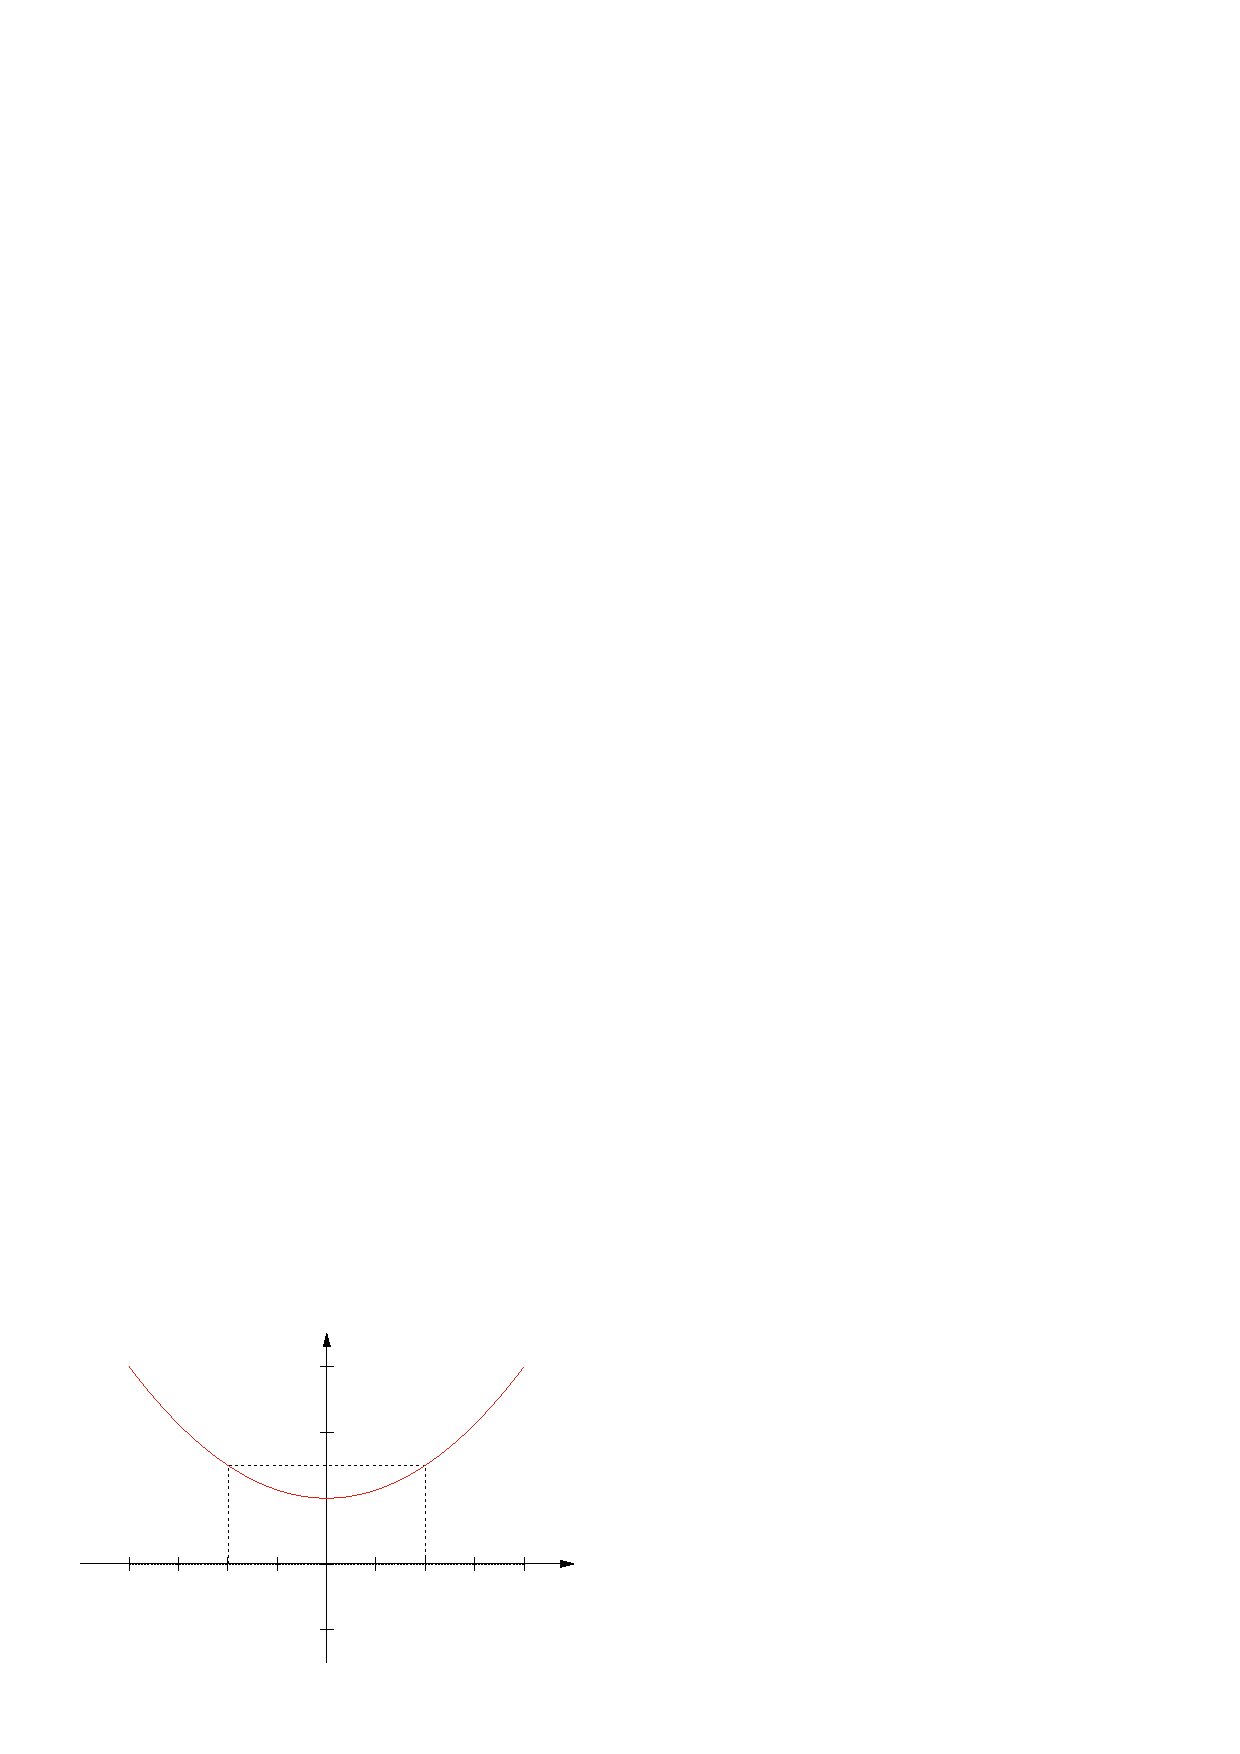
\includegraphics[width={216.00bp},height={144.00bp}]{figura_02_01}}%
    \gplfronttext
  \end{picture}%
\endgroup

    \caption{La gráfica se refleja \\respecto al eje central.}
\end{figure}

\textbf{Ejemplo 1:}
\begin{equation*}
    f(t)=t^2
\end{equation*}
\begin{equation*}
    f(-t)={(-t)}^2=t^2=f(t)
\end{equation*}

\textbf{Ejemplo 2:}
\begin{equation*}
    f(t)=\cos(t)
\end{equation*}
\begin{equation*}
    f(t)=\cos(-t)=\cos(t)=f(t)
\end{equation*}

Una función es \textbf{impar} si:
\begin{equation}
    f(-t)=-f(t)
\end{equation}
\begin{figure}[H]
    \centering
    % GNUPLOT: LaTeX picture with Postscript
\begingroup
  \makeatletter
  \providecommand\color[2][]{%
    \GenericError{(gnuplot) \space\space\space\@spaces}{%
      Package color not loaded in conjunction with
      terminal option `colourtext'%
    }{See the gnuplot documentation for explanation.%
    }{Either use 'blacktext' in gnuplot or load the package
      color.sty in LaTeX.}%
    \renewcommand\color[2][]{}%
  }%
  \providecommand\includegraphics[2][]{%
    \GenericError{(gnuplot) \space\space\space\@spaces}{%
      Package graphicx or graphics not loaded%
    }{See the gnuplot documentation for explanation.%
    }{The gnuplot epslatex terminal needs graphicx.sty or graphics.sty.}%
    \renewcommand\includegraphics[2][]{}%
  }%
  \providecommand\rotatebox[2]{#2}%
  \@ifundefined{ifGPcolor}{%
    \newif\ifGPcolor
    \GPcolorfalse
  }{}%
  \@ifundefined{ifGPblacktext}{%
    \newif\ifGPblacktext
    \GPblacktexttrue
  }{}%
  % define a \g@addto@macro without @ in the name:
  \let\gplgaddtomacro\g@addto@macro
  % define empty templates for all commands taking text:
  \gdef\gplbacktext{}%
  \gdef\gplfronttext{}%
  \makeatother
  \ifGPblacktext
    % no textcolor at all
    \def\colorrgb#1{}%
    \def\colorgray#1{}%
  \else
    % gray or color?
    \ifGPcolor
      \def\colorrgb#1{\color[rgb]{#1}}%
      \def\colorgray#1{\color[gray]{#1}}%
      \expandafter\def\csname LTw\endcsname{\color{white}}%
      \expandafter\def\csname LTb\endcsname{\color{black}}%
      \expandafter\def\csname LTa\endcsname{\color{black}}%
      \expandafter\def\csname LT0\endcsname{\color[rgb]{1,0,0}}%
      \expandafter\def\csname LT1\endcsname{\color[rgb]{0,1,0}}%
      \expandafter\def\csname LT2\endcsname{\color[rgb]{0,0,1}}%
      \expandafter\def\csname LT3\endcsname{\color[rgb]{1,0,1}}%
      \expandafter\def\csname LT4\endcsname{\color[rgb]{0,1,1}}%
      \expandafter\def\csname LT5\endcsname{\color[rgb]{1,1,0}}%
      \expandafter\def\csname LT6\endcsname{\color[rgb]{0,0,0}}%
      \expandafter\def\csname LT7\endcsname{\color[rgb]{1,0.3,0}}%
      \expandafter\def\csname LT8\endcsname{\color[rgb]{0.5,0.5,0.5}}%
    \else
      % gray
      \def\colorrgb#1{\color{black}}%
      \def\colorgray#1{\color[gray]{#1}}%
      \expandafter\def\csname LTw\endcsname{\color{white}}%
      \expandafter\def\csname LTb\endcsname{\color{black}}%
      \expandafter\def\csname LTa\endcsname{\color{black}}%
      \expandafter\def\csname LT0\endcsname{\color{black}}%
      \expandafter\def\csname LT1\endcsname{\color{black}}%
      \expandafter\def\csname LT2\endcsname{\color{black}}%
      \expandafter\def\csname LT3\endcsname{\color{black}}%
      \expandafter\def\csname LT4\endcsname{\color{black}}%
      \expandafter\def\csname LT5\endcsname{\color{black}}%
      \expandafter\def\csname LT6\endcsname{\color{black}}%
      \expandafter\def\csname LT7\endcsname{\color{black}}%
      \expandafter\def\csname LT8\endcsname{\color{black}}%
    \fi
  \fi
    \setlength{\unitlength}{0.0500bp}%
    \ifx\gptboxheight\undefined%
      \newlength{\gptboxheight}%
      \newlength{\gptboxwidth}%
      \newsavebox{\gptboxtext}%
    \fi%
    \setlength{\fboxrule}{0.5pt}%
    \setlength{\fboxsep}{1pt}%
    \definecolor{tbcol}{rgb}{1,1,1}%
\begin{picture}(4320.00,2880.00)%
    \gplgaddtomacro\gplbacktext{%
      \csname LTb\endcsname%%
      \put(2040,192){\makebox(0,0)[r]{\strut{}}}%
      \put(2040,824){\makebox(0,0)[r]{\strut{}}}%
      \put(2040,1456){\makebox(0,0)[r]{\strut{}}}%
      \put(2040,2087){\makebox(0,0)[r]{\strut{}}}%
      \put(2040,2719){\makebox(0,0)[r]{\strut{}}}%
      \put(240,1233){\makebox(0,0){\strut{}}}%
      \put(714,1233){\makebox(0,0){\strut{}}}%
      \put(1188,1233){\makebox(0,0){\strut{}}}%
      \put(1662,1233){\makebox(0,0){\strut{}}}%
      \put(2136,1233){\makebox(0,0){\strut{}}}%
      \put(2609,1233){\makebox(0,0){\strut{}}}%
      \put(3083,1233){\makebox(0,0){\strut{}}}%
      \put(3557,1233){\makebox(0,0){\strut{}}}%
      \put(4031,1233){\makebox(0,0){\strut{}}}%
      \csname LTb\endcsname%%
      \put(4647,1456){\makebox(0,0)[l]{\strut{}$t$}}%
      \put(2349,2845){\makebox(0,0)[l]{\strut{}$f(t)$}}%
      \put(998,1645){\makebox(0,0)[l]{\strut{}$-t_1$}}%
      \put(3036,1266){\makebox(0,0)[l]{\strut{}$ t_1$}}%
      \put(2372,824){\makebox(0,0)[l]{\strut{}$-f(t_1)=f(-t_1)$}}%
    }%
    \gplgaddtomacro\gplfronttext{%
    }%
    \gplbacktext
    \put(0,0){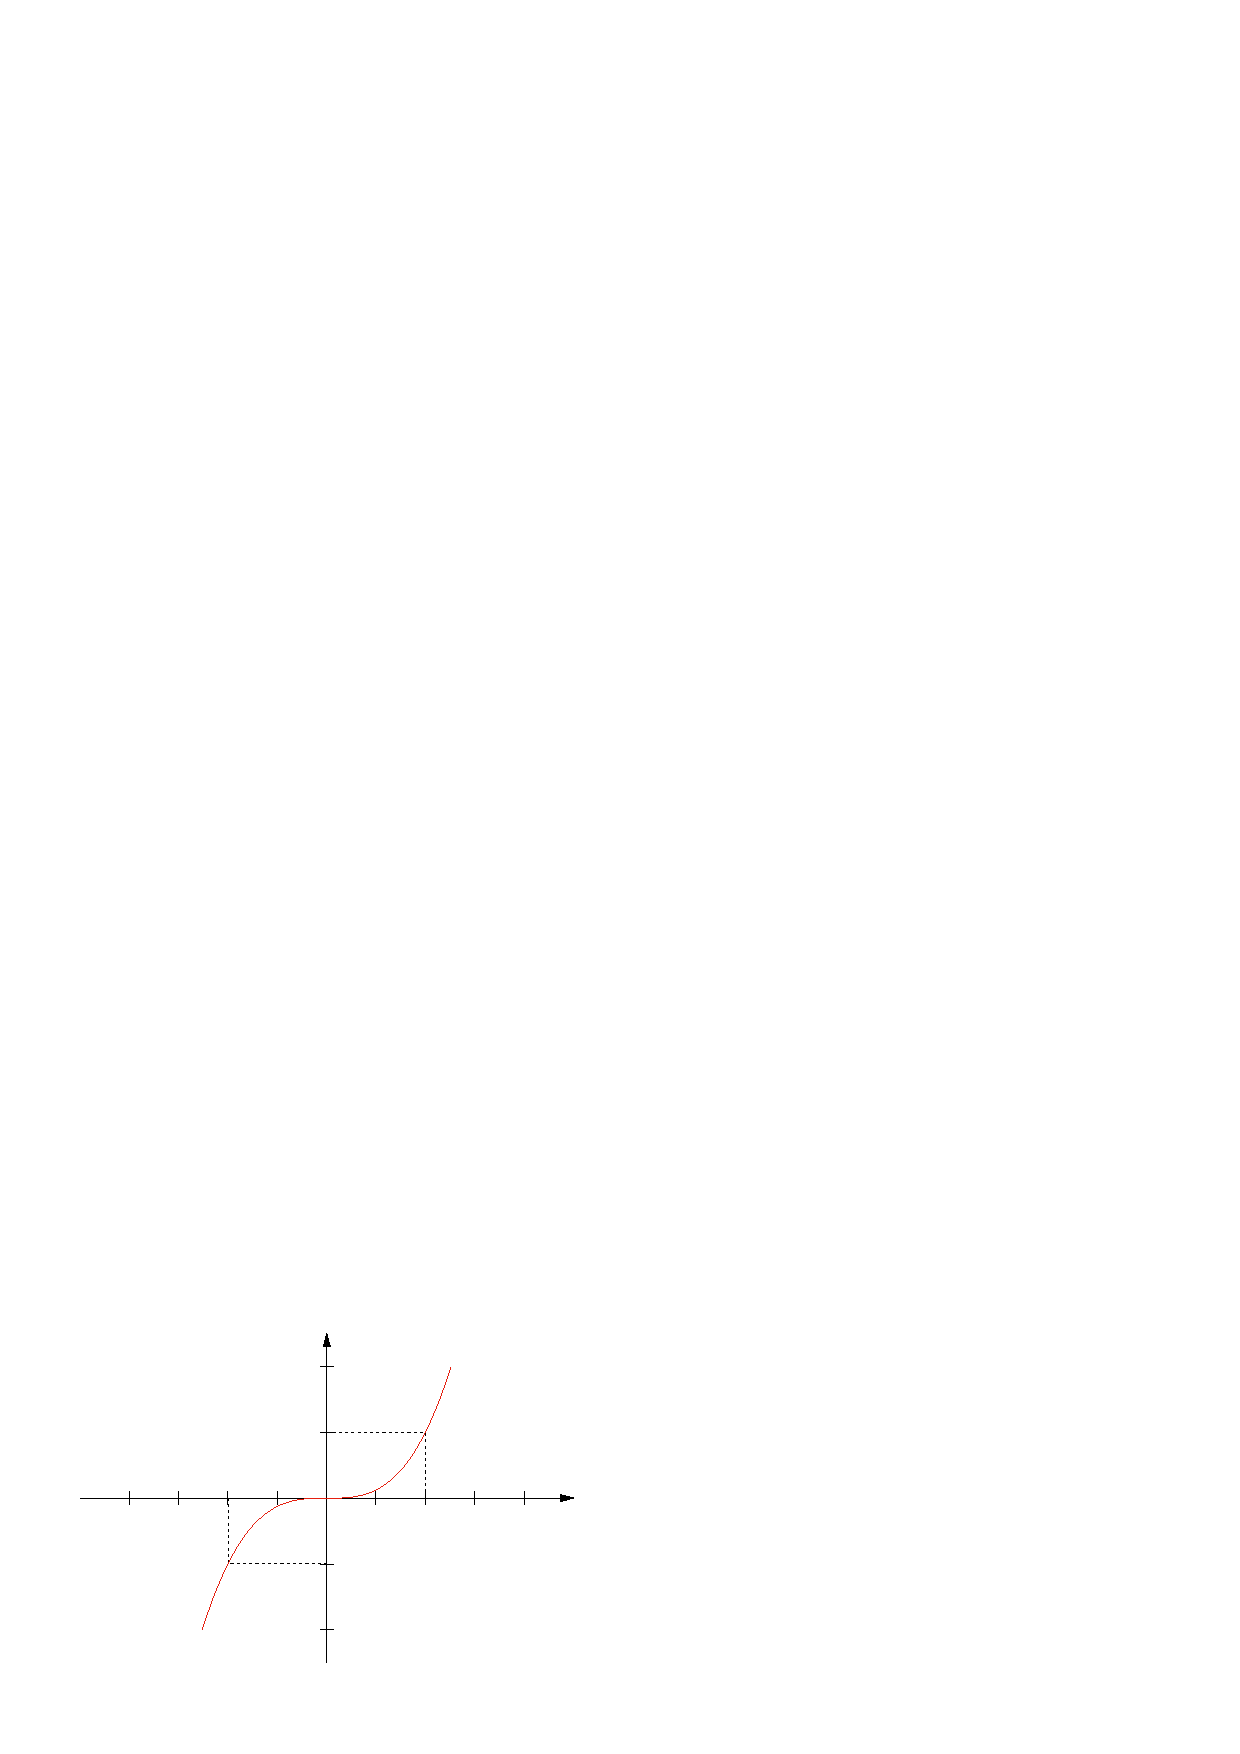
\includegraphics[width={216.00bp},height={144.00bp}]{figura_02_02}}%
    \gplfronttext
  \end{picture}%
\endgroup

    \caption{La gráfica se refleja \\
    1ro respecto al eje central\\
    2do respecto al eje horizontal.}
\end{figure}

\textbf{Ejemplo 3:}
\begin{equation*}
    f(t)=t^3
\end{equation*}
\begin{equation*}
    f(-t)={(-t)}^3=-t^3=-f(t)
\end{equation*}

\textbf{Ejemplo 4:}
\begin{equation*}
    f(t)=\sen(t)
\end{equation*}
\begin{equation*}
    f(t)=\sen(-t)=-\sen(t)=-f(t)
\end{equation*}

\textbf{Ejemplo 5:}
\begin{equation*}
    f(t)=\begin{cases}
        e^t &t<0\\
        e^{-t} &t>0\\
    \end{cases}
\end{equation*}
\begin{equation*}
    f(-t)=\left\{\!\begin{aligned}
    &e^{-t} &-t<0 \rightarrow t>0\\
    &e^{t}  &-t>0 \rightarrow t<0\\
    \end{aligned}\right\}
    =f(t)
\end{equation*}
\begin{figure}[H]
    \centering
    % GNUPLOT: LaTeX picture with Postscript
\begingroup
  \makeatletter
  \providecommand\color[2][]{%
    \GenericError{(gnuplot) \space\space\space\@spaces}{%
      Package color not loaded in conjunction with
      terminal option `colourtext'%
    }{See the gnuplot documentation for explanation.%
    }{Either use 'blacktext' in gnuplot or load the package
      color.sty in LaTeX.}%
    \renewcommand\color[2][]{}%
  }%
  \providecommand\includegraphics[2][]{%
    \GenericError{(gnuplot) \space\space\space\@spaces}{%
      Package graphicx or graphics not loaded%
    }{See the gnuplot documentation for explanation.%
    }{The gnuplot epslatex terminal needs graphicx.sty or graphics.sty.}%
    \renewcommand\includegraphics[2][]{}%
  }%
  \providecommand\rotatebox[2]{#2}%
  \@ifundefined{ifGPcolor}{%
    \newif\ifGPcolor
    \GPcolorfalse
  }{}%
  \@ifundefined{ifGPblacktext}{%
    \newif\ifGPblacktext
    \GPblacktexttrue
  }{}%
  % define a \g@addto@macro without @ in the name:
  \let\gplgaddtomacro\g@addto@macro
  % define empty templates for all commands taking text:
  \gdef\gplbacktext{}%
  \gdef\gplfronttext{}%
  \makeatother
  \ifGPblacktext
    % no textcolor at all
    \def\colorrgb#1{}%
    \def\colorgray#1{}%
  \else
    % gray or color?
    \ifGPcolor
      \def\colorrgb#1{\color[rgb]{#1}}%
      \def\colorgray#1{\color[gray]{#1}}%
      \expandafter\def\csname LTw\endcsname{\color{white}}%
      \expandafter\def\csname LTb\endcsname{\color{black}}%
      \expandafter\def\csname LTa\endcsname{\color{black}}%
      \expandafter\def\csname LT0\endcsname{\color[rgb]{1,0,0}}%
      \expandafter\def\csname LT1\endcsname{\color[rgb]{0,1,0}}%
      \expandafter\def\csname LT2\endcsname{\color[rgb]{0,0,1}}%
      \expandafter\def\csname LT3\endcsname{\color[rgb]{1,0,1}}%
      \expandafter\def\csname LT4\endcsname{\color[rgb]{0,1,1}}%
      \expandafter\def\csname LT5\endcsname{\color[rgb]{1,1,0}}%
      \expandafter\def\csname LT6\endcsname{\color[rgb]{0,0,0}}%
      \expandafter\def\csname LT7\endcsname{\color[rgb]{1,0.3,0}}%
      \expandafter\def\csname LT8\endcsname{\color[rgb]{0.5,0.5,0.5}}%
    \else
      % gray
      \def\colorrgb#1{\color{black}}%
      \def\colorgray#1{\color[gray]{#1}}%
      \expandafter\def\csname LTw\endcsname{\color{white}}%
      \expandafter\def\csname LTb\endcsname{\color{black}}%
      \expandafter\def\csname LTa\endcsname{\color{black}}%
      \expandafter\def\csname LT0\endcsname{\color{black}}%
      \expandafter\def\csname LT1\endcsname{\color{black}}%
      \expandafter\def\csname LT2\endcsname{\color{black}}%
      \expandafter\def\csname LT3\endcsname{\color{black}}%
      \expandafter\def\csname LT4\endcsname{\color{black}}%
      \expandafter\def\csname LT5\endcsname{\color{black}}%
      \expandafter\def\csname LT6\endcsname{\color{black}}%
      \expandafter\def\csname LT7\endcsname{\color{black}}%
      \expandafter\def\csname LT8\endcsname{\color{black}}%
    \fi
  \fi
    \setlength{\unitlength}{0.0500bp}%
    \ifx\gptboxheight\undefined%
      \newlength{\gptboxheight}%
      \newlength{\gptboxwidth}%
      \newsavebox{\gptboxtext}%
    \fi%
    \setlength{\fboxrule}{0.5pt}%
    \setlength{\fboxsep}{1pt}%
    \definecolor{tbcol}{rgb}{1,1,1}%
\begin{picture}(5760.00,1440.00)%
    \gplgaddtomacro\gplbacktext{%
      \csname LTb\endcsname%%
      \put(2760,464){\makebox(0,0)[r]{\strut{}}}%
      \put(2760,1007){\makebox(0,0)[r]{\strut{}}}%
      \put(240,241){\makebox(0,0){\strut{}}}%
      \put(763,241){\makebox(0,0){\strut{}}}%
      \put(1286,241){\makebox(0,0){\strut{}}}%
      \put(1809,241){\makebox(0,0){\strut{}}}%
      \put(2332,241){\makebox(0,0){\strut{}}}%
      \put(2856,241){\makebox(0,0){\strut{}}}%
      \put(3379,241){\makebox(0,0){\strut{}}}%
      \put(3902,241){\makebox(0,0){\strut{}}}%
      \put(4425,241){\makebox(0,0){\strut{}}}%
      \put(4948,241){\makebox(0,0){\strut{}}}%
      \put(5471,241){\makebox(0,0){\strut{}}}%
      \csname LTb\endcsname%%
      \put(6256,464){\makebox(0,0)[l]{\strut{}$t$}}%
      \put(2751,1496){\makebox(0,0)[l]{\strut{}$f(t)$}}%
    }%
    \gplgaddtomacro\gplfronttext{%
    }%
    \gplgaddtomacro\gplbacktext{%
      \csname LTb\endcsname%%
      \put(2760,464){\makebox(0,0)[r]{\strut{}}}%
      \put(2760,1007){\makebox(0,0)[r]{\strut{}}}%
      \put(240,241){\makebox(0,0){\strut{}}}%
      \put(763,241){\makebox(0,0){\strut{}}}%
      \put(1286,241){\makebox(0,0){\strut{}}}%
      \put(1809,241){\makebox(0,0){\strut{}}}%
      \put(2332,241){\makebox(0,0){\strut{}}}%
      \put(2856,241){\makebox(0,0){\strut{}}}%
      \put(3379,241){\makebox(0,0){\strut{}}}%
      \put(3902,241){\makebox(0,0){\strut{}}}%
      \put(4425,241){\makebox(0,0){\strut{}}}%
      \put(4948,241){\makebox(0,0){\strut{}}}%
      \put(5471,241){\makebox(0,0){\strut{}}}%
      \csname LTb\endcsname%%
      \put(6256,464){\makebox(0,0)[l]{\strut{}$t$}}%
      \put(2751,1496){\makebox(0,0)[l]{\strut{}$f(t)$}}%
    }%
    \gplgaddtomacro\gplfronttext{%
    }%
    \gplbacktext
    \put(0,0){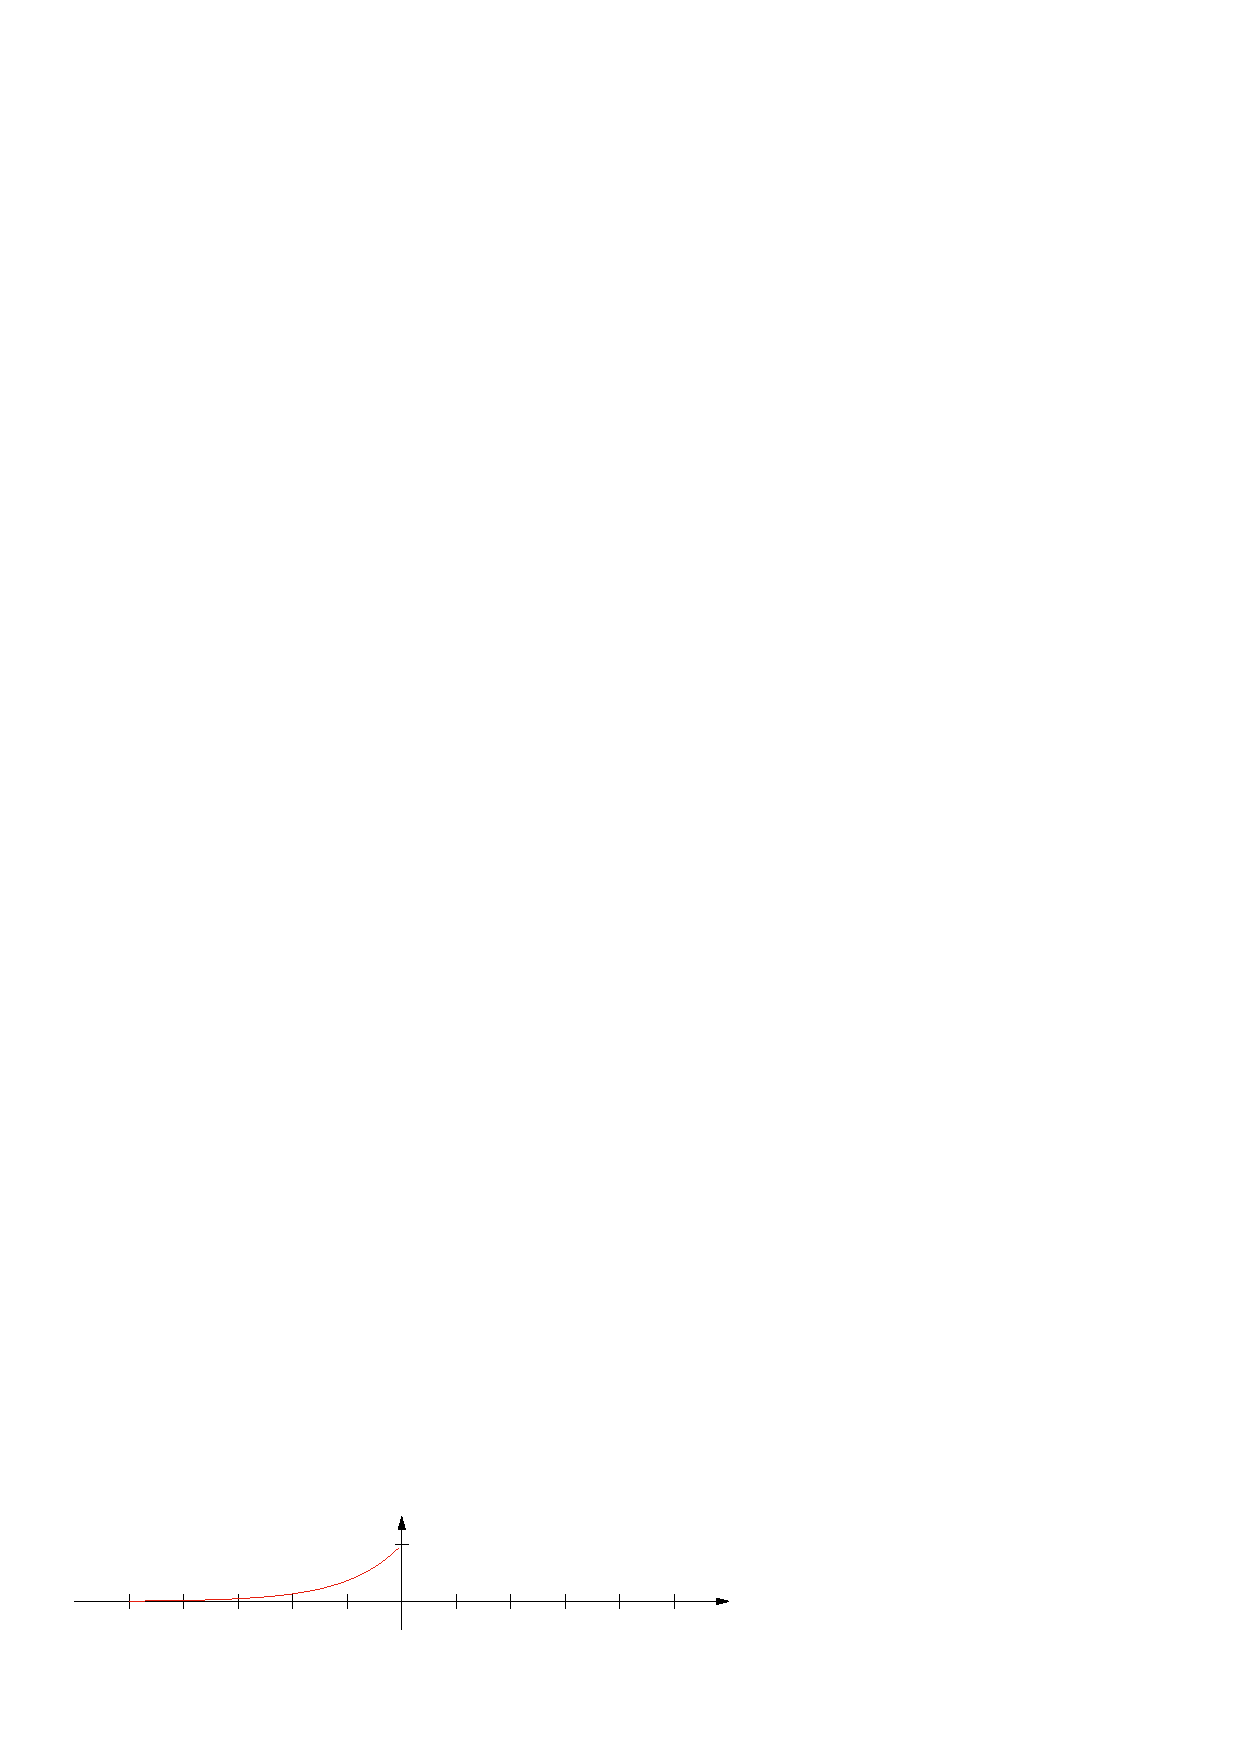
\includegraphics[width={288.00bp},height={72.00bp}]{figura_02_03}}%
    \gplfronttext
  \end{picture}%
\endgroup

\end{figure}

\subsection{Propiedades de las funciones pares e impares}
\subsubsection*{Propiedad 1}
Si $f(t)$ es \textbf{par} y $g(t)$ es \textbf{par}, entonces $h(t)=f(t)g(t)$ es
\textbf{par}.

\underline{Prueba}:
\begin{equation*}
\begin{cases}
    &f(-t)=f(t)\\
    &g(-t)=g(t)\\
\end{cases}
\end{equation*}
\begin{equation*}
\begin{split}
    h(-t)
        &=f(-t)g(-t)\\
        &=f(t)g(t)\\
        &=h(t)\\
\end{split}
\end{equation*}

\subsubsection*{Propiedad 2}
Si $f(t)$ es \textbf{impar} y $g(t)$ es \textbf{impar}, entonces $h(t)=f(t)g(t)$
es \textbf{par}.

\underline{Prueba}:
\begin{equation*}
\begin{cases}
    &f(-t)=-f(t)\\
    &g(-t)=-g(t)\\
\end{cases}
\end{equation*}

\subsubsection*{Propiedad 3}
Si $f(t)$ es \textbf{par} y $g(t)$ es \textbf{impar}, entonces $h(t)=f(t)g(t)$
es \textbf{impar}.

\underline{Prueba}:
\begin{equation*}
\begin{cases}
    &f(-t)=f(t)\\
    &g(-t)=-g(t)\\
\end{cases}
\end{equation*}
\begin{equation*}
\begin{split}
    h(-t)
        &=f(-t)g(-t)\\
        &=f(t)(-g(t))\\
        &=-f(t)g(t)\\
        &=-h(t)\\
\end{split}
\end{equation*}

\subsubsection*{Propiedad 4}
Si $f(t)$ es \textbf{par}, entonces:
\begin{equation}
    \int_{-a}^a f(t)\,dt=2\int_0^a f(t)\,dt
\end{equation}
\begin{figure}[H]
    \centering
    % GNUPLOT: LaTeX picture with Postscript
\begingroup
  \makeatletter
  \providecommand\color[2][]{%
    \GenericError{(gnuplot) \space\space\space\@spaces}{%
      Package color not loaded in conjunction with
      terminal option `colourtext'%
    }{See the gnuplot documentation for explanation.%
    }{Either use 'blacktext' in gnuplot or load the package
      color.sty in LaTeX.}%
    \renewcommand\color[2][]{}%
  }%
  \providecommand\includegraphics[2][]{%
    \GenericError{(gnuplot) \space\space\space\@spaces}{%
      Package graphicx or graphics not loaded%
    }{See the gnuplot documentation for explanation.%
    }{The gnuplot epslatex terminal needs graphicx.sty or graphics.sty.}%
    \renewcommand\includegraphics[2][]{}%
  }%
  \providecommand\rotatebox[2]{#2}%
  \@ifundefined{ifGPcolor}{%
    \newif\ifGPcolor
    \GPcolorfalse
  }{}%
  \@ifundefined{ifGPblacktext}{%
    \newif\ifGPblacktext
    \GPblacktexttrue
  }{}%
  % define a \g@addto@macro without @ in the name:
  \let\gplgaddtomacro\g@addto@macro
  % define empty templates for all commands taking text:
  \gdef\gplbacktext{}%
  \gdef\gplfronttext{}%
  \makeatother
  \ifGPblacktext
    % no textcolor at all
    \def\colorrgb#1{}%
    \def\colorgray#1{}%
  \else
    % gray or color?
    \ifGPcolor
      \def\colorrgb#1{\color[rgb]{#1}}%
      \def\colorgray#1{\color[gray]{#1}}%
      \expandafter\def\csname LTw\endcsname{\color{white}}%
      \expandafter\def\csname LTb\endcsname{\color{black}}%
      \expandafter\def\csname LTa\endcsname{\color{black}}%
      \expandafter\def\csname LT0\endcsname{\color[rgb]{1,0,0}}%
      \expandafter\def\csname LT1\endcsname{\color[rgb]{0,1,0}}%
      \expandafter\def\csname LT2\endcsname{\color[rgb]{0,0,1}}%
      \expandafter\def\csname LT3\endcsname{\color[rgb]{1,0,1}}%
      \expandafter\def\csname LT4\endcsname{\color[rgb]{0,1,1}}%
      \expandafter\def\csname LT5\endcsname{\color[rgb]{1,1,0}}%
      \expandafter\def\csname LT6\endcsname{\color[rgb]{0,0,0}}%
      \expandafter\def\csname LT7\endcsname{\color[rgb]{1,0.3,0}}%
      \expandafter\def\csname LT8\endcsname{\color[rgb]{0.5,0.5,0.5}}%
    \else
      % gray
      \def\colorrgb#1{\color{black}}%
      \def\colorgray#1{\color[gray]{#1}}%
      \expandafter\def\csname LTw\endcsname{\color{white}}%
      \expandafter\def\csname LTb\endcsname{\color{black}}%
      \expandafter\def\csname LTa\endcsname{\color{black}}%
      \expandafter\def\csname LT0\endcsname{\color{black}}%
      \expandafter\def\csname LT1\endcsname{\color{black}}%
      \expandafter\def\csname LT2\endcsname{\color{black}}%
      \expandafter\def\csname LT3\endcsname{\color{black}}%
      \expandafter\def\csname LT4\endcsname{\color{black}}%
      \expandafter\def\csname LT5\endcsname{\color{black}}%
      \expandafter\def\csname LT6\endcsname{\color{black}}%
      \expandafter\def\csname LT7\endcsname{\color{black}}%
      \expandafter\def\csname LT8\endcsname{\color{black}}%
    \fi
  \fi
    \setlength{\unitlength}{0.0500bp}%
    \ifx\gptboxheight\undefined%
      \newlength{\gptboxheight}%
      \newlength{\gptboxwidth}%
      \newsavebox{\gptboxtext}%
    \fi%
    \setlength{\fboxrule}{0.5pt}%
    \setlength{\fboxsep}{1pt}%
    \definecolor{tbcol}{rgb}{1,1,1}%
\begin{picture}(4320.00,2880.00)%
    \gplgaddtomacro\gplbacktext{%
      \csname LTb\endcsname%%
      \put(2040,192){\makebox(0,0)[r]{\strut{}}}%
      \put(2040,824){\makebox(0,0)[r]{\strut{}}}%
      \put(2040,1456){\makebox(0,0)[r]{\strut{}}}%
      \put(2040,2087){\makebox(0,0)[r]{\strut{}}}%
      \put(2040,2719){\makebox(0,0)[r]{\strut{}}}%
      \put(240,601){\makebox(0,0){\strut{}}}%
      \put(714,601){\makebox(0,0){\strut{}}}%
      \put(1188,601){\makebox(0,0){\strut{}}}%
      \put(1662,601){\makebox(0,0){\strut{}}}%
      \put(2136,601){\makebox(0,0){\strut{}}}%
      \put(2609,601){\makebox(0,0){\strut{}}}%
      \put(3083,601){\makebox(0,0){\strut{}}}%
      \put(3557,601){\makebox(0,0){\strut{}}}%
      \put(4031,601){\makebox(0,0){\strut{}}}%
      \csname LTb\endcsname%%
      \put(4647,824){\makebox(0,0)[l]{\strut{}$t$}}%
      \put(2349,2972){\makebox(0,0)[l]{\strut{}$f(t)$}}%
      \put(998,634){\makebox(0,0)[l]{\strut{}$-a$}}%
      \put(3036,634){\makebox(0,0)[l]{\strut{}$ a$}}%
      \put(3557,1456){\makebox(0,0)[l]{\strut{}$\int_0^a f(t)dt$}}%
    }%
    \gplgaddtomacro\gplfronttext{%
    }%
    \gplgaddtomacro\gplbacktext{%
      \csname LTb\endcsname%%
      \put(2040,192){\makebox(0,0)[r]{\strut{}}}%
      \put(2040,824){\makebox(0,0)[r]{\strut{}}}%
      \put(2040,1456){\makebox(0,0)[r]{\strut{}}}%
      \put(2040,2087){\makebox(0,0)[r]{\strut{}}}%
      \put(2040,2719){\makebox(0,0)[r]{\strut{}}}%
      \put(240,601){\makebox(0,0){\strut{}}}%
      \put(714,601){\makebox(0,0){\strut{}}}%
      \put(1188,601){\makebox(0,0){\strut{}}}%
      \put(1662,601){\makebox(0,0){\strut{}}}%
      \put(2136,601){\makebox(0,0){\strut{}}}%
      \put(2609,601){\makebox(0,0){\strut{}}}%
      \put(3083,601){\makebox(0,0){\strut{}}}%
      \put(3557,601){\makebox(0,0){\strut{}}}%
      \put(4031,601){\makebox(0,0){\strut{}}}%
      \csname LTb\endcsname%%
      \put(4647,824){\makebox(0,0)[l]{\strut{}$t$}}%
      \put(2349,2972){\makebox(0,0)[l]{\strut{}$f(t)$}}%
      \put(998,634){\makebox(0,0)[l]{\strut{}$-a$}}%
      \put(3036,634){\makebox(0,0)[l]{\strut{}$ a$}}%
      \put(3557,1456){\makebox(0,0)[l]{\strut{}$\int_0^a f(t)dt$}}%
    }%
    \gplgaddtomacro\gplfronttext{%
    }%
    \gplgaddtomacro\gplbacktext{%
      \csname LTb\endcsname%%
      \put(2040,192){\makebox(0,0)[r]{\strut{}}}%
      \put(2040,824){\makebox(0,0)[r]{\strut{}}}%
      \put(2040,1456){\makebox(0,0)[r]{\strut{}}}%
      \put(2040,2087){\makebox(0,0)[r]{\strut{}}}%
      \put(2040,2719){\makebox(0,0)[r]{\strut{}}}%
      \put(240,601){\makebox(0,0){\strut{}}}%
      \put(714,601){\makebox(0,0){\strut{}}}%
      \put(1188,601){\makebox(0,0){\strut{}}}%
      \put(1662,601){\makebox(0,0){\strut{}}}%
      \put(2136,601){\makebox(0,0){\strut{}}}%
      \put(2609,601){\makebox(0,0){\strut{}}}%
      \put(3083,601){\makebox(0,0){\strut{}}}%
      \put(3557,601){\makebox(0,0){\strut{}}}%
      \put(4031,601){\makebox(0,0){\strut{}}}%
      \csname LTb\endcsname%%
      \put(4647,824){\makebox(0,0)[l]{\strut{}$t$}}%
      \put(2349,2972){\makebox(0,0)[l]{\strut{}$f(t)$}}%
      \put(998,634){\makebox(0,0)[l]{\strut{}$-a$}}%
      \put(3036,634){\makebox(0,0)[l]{\strut{}$ a$}}%
      \put(3557,1456){\makebox(0,0)[l]{\strut{}$\int_0^a f(t)dt$}}%
    }%
    \gplgaddtomacro\gplfronttext{%
    }%
    \gplbacktext
    \put(0,0){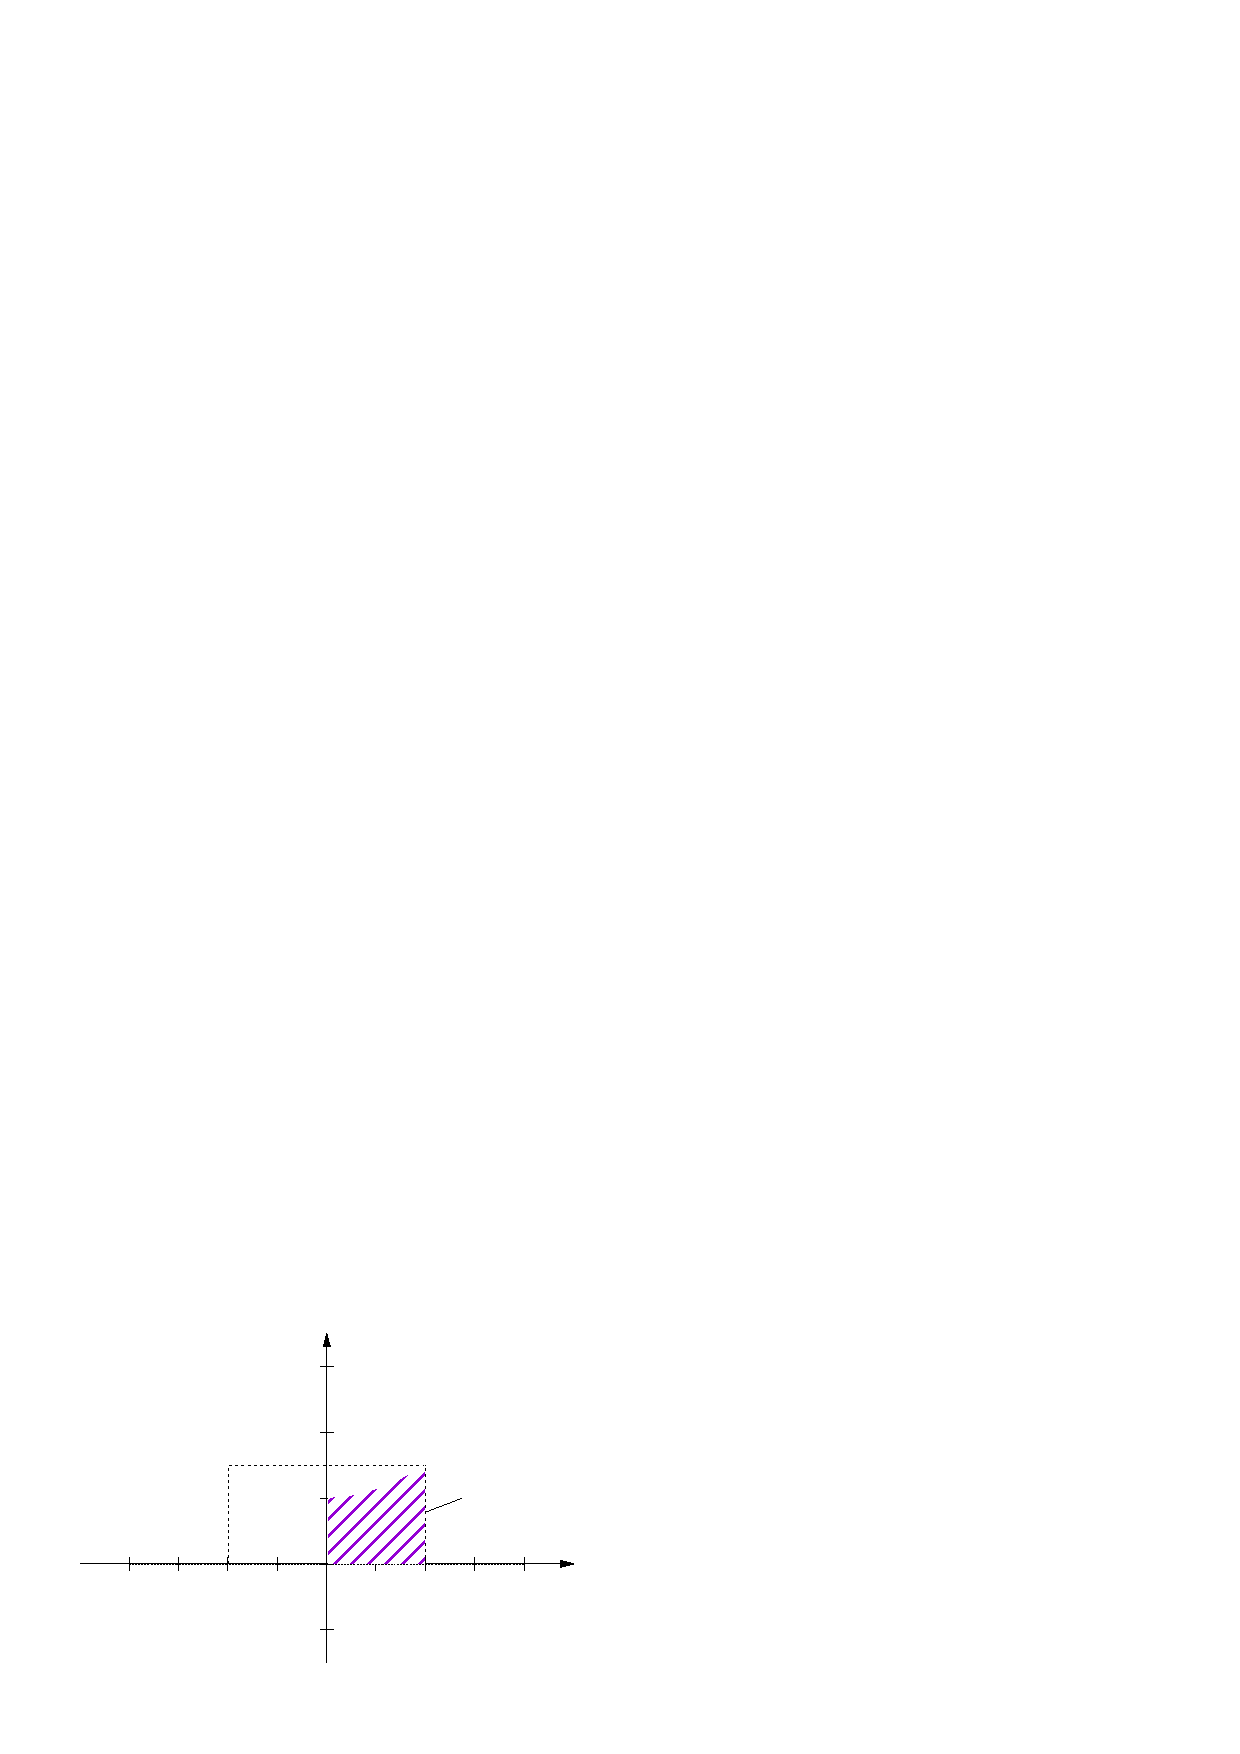
\includegraphics[width={216.00bp},height={144.00bp}]{figura_02_04}}%
    \gplfronttext
  \end{picture}%
\endgroup

\end{figure}

\underline{Prueba}:
\begin{equation*}
\begin{split}
    \int_{-a}^a f(t)\,dt
        &=\int_{-a}^0 f(t)\,dt+\int_0^a f(t)\,dt\\
        &=\int_{-a}^0 f(-t)\,dt+\int_0^a f(t)\,dt\\
\end{split}
\end{equation*}
\begin{equation*}
    \tau=-t
\end{equation*}
\begin{equation*}
    d\tau=-dt
\end{equation*}
\begin{equation*}
\begin{split}
    \int_{-a}^a f(t)\,dt
        &=\int_a^0 f(\tau)\,(-d\tau)+\int_0^a f(t)\,dt\\
        &=\int_0^a f(\tau)\,d\tau+\int_0^a f(t)\,dt\\
        &=2\int_0^a f(t)\,dt\\
\end{split}
\end{equation*}

\subsubsection*{Propiedad 5}
Si $f(t)$ es \textbf{impar}, entonces:
\begin{equation}
    \int_{-a}^a f(t)\,dt=0
\end{equation}
\begin{figure}[H]
    \centering
    % GNUPLOT: LaTeX picture with Postscript
\begingroup
  \makeatletter
  \providecommand\color[2][]{%
    \GenericError{(gnuplot) \space\space\space\@spaces}{%
      Package color not loaded in conjunction with
      terminal option `colourtext'%
    }{See the gnuplot documentation for explanation.%
    }{Either use 'blacktext' in gnuplot or load the package
      color.sty in LaTeX.}%
    \renewcommand\color[2][]{}%
  }%
  \providecommand\includegraphics[2][]{%
    \GenericError{(gnuplot) \space\space\space\@spaces}{%
      Package graphicx or graphics not loaded%
    }{See the gnuplot documentation for explanation.%
    }{The gnuplot epslatex terminal needs graphicx.sty or graphics.sty.}%
    \renewcommand\includegraphics[2][]{}%
  }%
  \providecommand\rotatebox[2]{#2}%
  \@ifundefined{ifGPcolor}{%
    \newif\ifGPcolor
    \GPcolorfalse
  }{}%
  \@ifundefined{ifGPblacktext}{%
    \newif\ifGPblacktext
    \GPblacktexttrue
  }{}%
  % define a \g@addto@macro without @ in the name:
  \let\gplgaddtomacro\g@addto@macro
  % define empty templates for all commands taking text:
  \gdef\gplbacktext{}%
  \gdef\gplfronttext{}%
  \makeatother
  \ifGPblacktext
    % no textcolor at all
    \def\colorrgb#1{}%
    \def\colorgray#1{}%
  \else
    % gray or color?
    \ifGPcolor
      \def\colorrgb#1{\color[rgb]{#1}}%
      \def\colorgray#1{\color[gray]{#1}}%
      \expandafter\def\csname LTw\endcsname{\color{white}}%
      \expandafter\def\csname LTb\endcsname{\color{black}}%
      \expandafter\def\csname LTa\endcsname{\color{black}}%
      \expandafter\def\csname LT0\endcsname{\color[rgb]{1,0,0}}%
      \expandafter\def\csname LT1\endcsname{\color[rgb]{0,1,0}}%
      \expandafter\def\csname LT2\endcsname{\color[rgb]{0,0,1}}%
      \expandafter\def\csname LT3\endcsname{\color[rgb]{1,0,1}}%
      \expandafter\def\csname LT4\endcsname{\color[rgb]{0,1,1}}%
      \expandafter\def\csname LT5\endcsname{\color[rgb]{1,1,0}}%
      \expandafter\def\csname LT6\endcsname{\color[rgb]{0,0,0}}%
      \expandafter\def\csname LT7\endcsname{\color[rgb]{1,0.3,0}}%
      \expandafter\def\csname LT8\endcsname{\color[rgb]{0.5,0.5,0.5}}%
    \else
      % gray
      \def\colorrgb#1{\color{black}}%
      \def\colorgray#1{\color[gray]{#1}}%
      \expandafter\def\csname LTw\endcsname{\color{white}}%
      \expandafter\def\csname LTb\endcsname{\color{black}}%
      \expandafter\def\csname LTa\endcsname{\color{black}}%
      \expandafter\def\csname LT0\endcsname{\color{black}}%
      \expandafter\def\csname LT1\endcsname{\color{black}}%
      \expandafter\def\csname LT2\endcsname{\color{black}}%
      \expandafter\def\csname LT3\endcsname{\color{black}}%
      \expandafter\def\csname LT4\endcsname{\color{black}}%
      \expandafter\def\csname LT5\endcsname{\color{black}}%
      \expandafter\def\csname LT6\endcsname{\color{black}}%
      \expandafter\def\csname LT7\endcsname{\color{black}}%
      \expandafter\def\csname LT8\endcsname{\color{black}}%
    \fi
  \fi
    \setlength{\unitlength}{0.0500bp}%
    \ifx\gptboxheight\undefined%
      \newlength{\gptboxheight}%
      \newlength{\gptboxwidth}%
      \newsavebox{\gptboxtext}%
    \fi%
    \setlength{\fboxrule}{0.5pt}%
    \setlength{\fboxsep}{1pt}%
    \definecolor{tbcol}{rgb}{1,1,1}%
\begin{picture}(4320.00,2880.00)%
    \gplgaddtomacro\gplbacktext{%
      \csname LTb\endcsname%%
      \put(2040,192){\makebox(0,0)[r]{\strut{}}}%
      \put(2040,824){\makebox(0,0)[r]{\strut{}}}%
      \put(2040,1456){\makebox(0,0)[r]{\strut{}}}%
      \put(2040,2087){\makebox(0,0)[r]{\strut{}}}%
      \put(2040,2719){\makebox(0,0)[r]{\strut{}}}%
      \put(240,1233){\makebox(0,0){\strut{}}}%
      \put(714,1233){\makebox(0,0){\strut{}}}%
      \put(1188,1233){\makebox(0,0){\strut{}}}%
      \put(1662,1233){\makebox(0,0){\strut{}}}%
      \put(2136,1233){\makebox(0,0){\strut{}}}%
      \put(2609,1233){\makebox(0,0){\strut{}}}%
      \put(3083,1233){\makebox(0,0){\strut{}}}%
      \put(3557,1233){\makebox(0,0){\strut{}}}%
      \put(4031,1233){\makebox(0,0){\strut{}}}%
      \csname LTb\endcsname%%
      \put(4647,1456){\makebox(0,0)[l]{\strut{}$t$}}%
      \put(2349,2845){\makebox(0,0)[l]{\strut{}$f(t)$}}%
      \put(998,1645){\makebox(0,0)[l]{\strut{}$-a$}}%
      \put(3036,1266){\makebox(0,0)[l]{\strut{}$ a$}}%
      \put(3557,2087){\makebox(0,0)[l]{\strut{}$\int_0^a f(t)dt$}}%
    }%
    \gplgaddtomacro\gplfronttext{%
    }%
    \gplgaddtomacro\gplbacktext{%
      \csname LTb\endcsname%%
      \put(2040,192){\makebox(0,0)[r]{\strut{}}}%
      \put(2040,824){\makebox(0,0)[r]{\strut{}}}%
      \put(2040,1456){\makebox(0,0)[r]{\strut{}}}%
      \put(2040,2087){\makebox(0,0)[r]{\strut{}}}%
      \put(2040,2719){\makebox(0,0)[r]{\strut{}}}%
      \put(240,1233){\makebox(0,0){\strut{}}}%
      \put(714,1233){\makebox(0,0){\strut{}}}%
      \put(1188,1233){\makebox(0,0){\strut{}}}%
      \put(1662,1233){\makebox(0,0){\strut{}}}%
      \put(2136,1233){\makebox(0,0){\strut{}}}%
      \put(2609,1233){\makebox(0,0){\strut{}}}%
      \put(3083,1233){\makebox(0,0){\strut{}}}%
      \put(3557,1233){\makebox(0,0){\strut{}}}%
      \put(4031,1233){\makebox(0,0){\strut{}}}%
      \csname LTb\endcsname%%
      \put(4647,1456){\makebox(0,0)[l]{\strut{}$t$}}%
      \put(2349,2845){\makebox(0,0)[l]{\strut{}$f(t)$}}%
      \put(998,1645){\makebox(0,0)[l]{\strut{}$-a$}}%
      \put(3036,1266){\makebox(0,0)[l]{\strut{}$ a$}}%
      \put(3557,2087){\makebox(0,0)[l]{\strut{}$\int_0^a f(t)dt$}}%
    }%
    \gplgaddtomacro\gplfronttext{%
    }%
    \gplgaddtomacro\gplbacktext{%
      \csname LTb\endcsname%%
      \put(2040,192){\makebox(0,0)[r]{\strut{}}}%
      \put(2040,824){\makebox(0,0)[r]{\strut{}}}%
      \put(2040,1456){\makebox(0,0)[r]{\strut{}}}%
      \put(2040,2087){\makebox(0,0)[r]{\strut{}}}%
      \put(2040,2719){\makebox(0,0)[r]{\strut{}}}%
      \put(240,1233){\makebox(0,0){\strut{}}}%
      \put(714,1233){\makebox(0,0){\strut{}}}%
      \put(1188,1233){\makebox(0,0){\strut{}}}%
      \put(1662,1233){\makebox(0,0){\strut{}}}%
      \put(2136,1233){\makebox(0,0){\strut{}}}%
      \put(2609,1233){\makebox(0,0){\strut{}}}%
      \put(3083,1233){\makebox(0,0){\strut{}}}%
      \put(3557,1233){\makebox(0,0){\strut{}}}%
      \put(4031,1233){\makebox(0,0){\strut{}}}%
      \csname LTb\endcsname%%
      \put(4647,1456){\makebox(0,0)[l]{\strut{}$t$}}%
      \put(2349,2845){\makebox(0,0)[l]{\strut{}$f(t)$}}%
      \put(998,1645){\makebox(0,0)[l]{\strut{}$-a$}}%
      \put(3036,1266){\makebox(0,0)[l]{\strut{}$ a$}}%
      \put(3557,2087){\makebox(0,0)[l]{\strut{}$\int_0^a f(t)dt$}}%
    }%
    \gplgaddtomacro\gplfronttext{%
    }%
    \gplbacktext
    \put(0,0){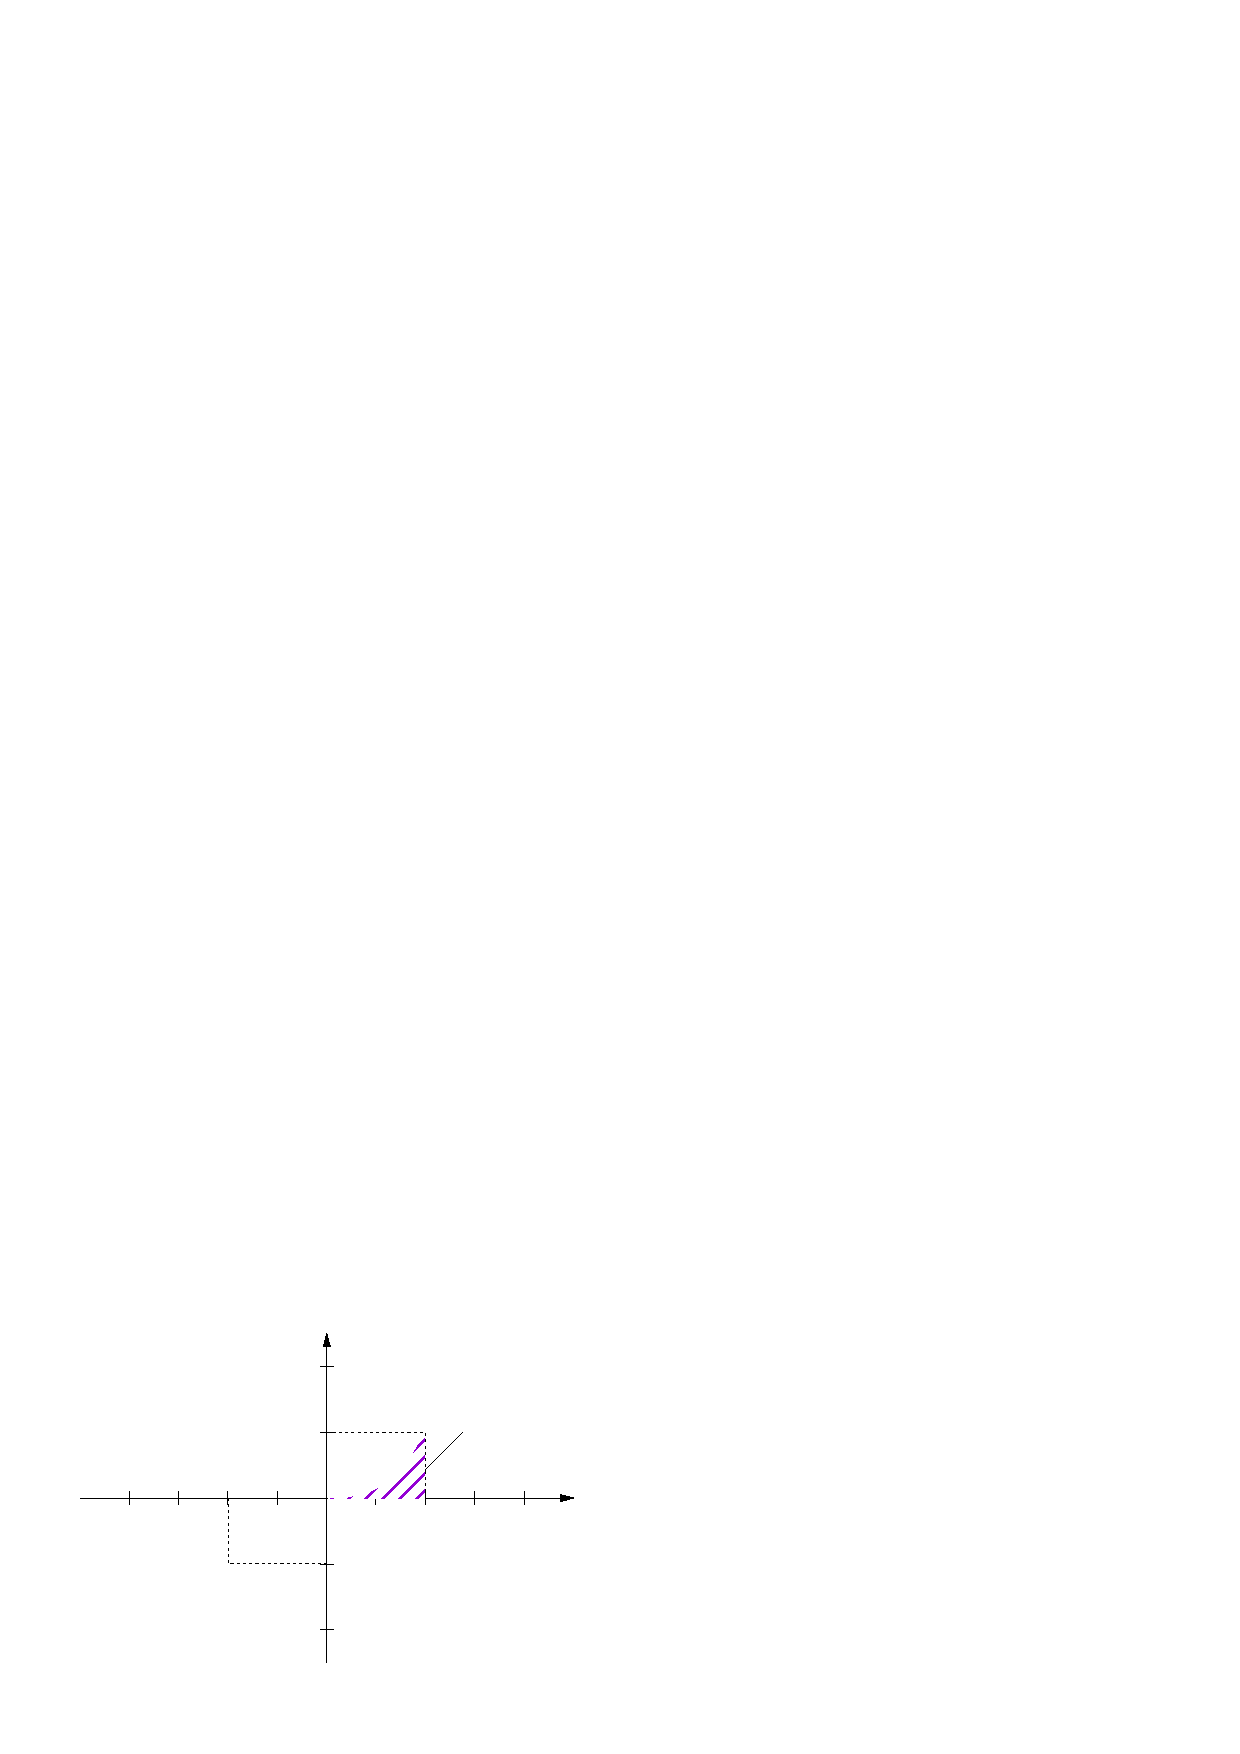
\includegraphics[width={216.00bp},height={144.00bp}]{figura_02_05}}%
    \gplfronttext
  \end{picture}%
\endgroup

\end{figure}

\underline{Prueba}:
\begin{equation*}
\begin{split}
    \int_{-a}^a f(t)\,dt
        &=\int_{-a}^0 f(t)\,dt+\int_0^a f(t)\,dt\\
        &=\int_{-a}^0 -f(-t)\,dt+\int_0^a f(t)\,dt\\
\end{split}
\end{equation*}
\begin{equation*}
    \tau=-t
\end{equation*}
\begin{equation*}
    d\tau=-dt
\end{equation*}
\begin{equation*}
\begin{split}
    \int_{-a}^a f(t)\,dt
        &=-\int_a^0 f(\tau)\,(-d\tau)+\int_0^a f(t)\,dt\\
        &=-\int_0^a f(\tau)\,d\tau+\int_0^a f(t)\,dt\\
        &=0\\
\end{split}
\end{equation*}

\subsection{Evaluación de coeficientes de \emph{Fourier}}
\subsubsection{Simetría par}
\begin{equation*}
\begin{split}
    a_0
        &=\frac{2}{T}\int_0^T f(t)\,dt\\
        &=\frac{2}{T}\int_{-T/2}^{T/2} f(t)\,dt\\
        &=\frac{2}{T}\left(2\int_0^{T/2} f(t)\,dt\right)\\
        &=\frac{4}{T}\int_0^{T/2} f(t)\,dt\\
\end{split}
\end{equation*}
\begin{equation}
    a_0=\frac{4}{T}\int_0^{T/2} f(t)\,dt
\end{equation}
\begin{equation*}
\begin{split}
    a_n
        &=\frac{2}{T}\int_{-T/2}^{T/2} f(t)\cos(n\omega_0 t)\,dt\\
        &=\frac{2}{T}\left(2\int_0^{T/2} f(t)\cos(n\omega_0 t)\,dt\right)\\
        &=\frac{4}{T}\int_0^{T/2}f(t)\cos(n\omega_0 t)\,dt\\
\end{split}
\end{equation*}
\begin{equation}
    a_n=\frac{4}{T}\int_0^{T/2}f(t)\cos(n\omega_0 t)\,dt
\end{equation}
\begin{equation*}
\begin{split}
    b_n
        &=\frac{2}{T}\int_{-T/2}^{T/2} f(t)\sen(n\omega_0 t)\,dt\\
        &=0\\
\end{split}
\end{equation*}
\begin{equation}
    b_n=0
\end{equation}

\subsubsection{Simetría impar}
\begin{equation*}
\begin{split}
    a_0
        &=\frac{2}{T}\int_0^T f(t)\,dt\\
        &=\frac{2}{T}\int_{-T/2}^{T/2} f(t)\,dt\\
        &=0\\
\end{split}
\end{equation*}
\begin{equation}
    a_0=0
\end{equation}
\begin{equation*}
\begin{split}
    a_n
        &=\frac{2}{T}\int_{-T/2}^{T/2} f(t)\cos(n\omega_0 t)\,dt\\
        &=0\\
\end{split}
\end{equation*}
\begin{equation}
    a_n=0
\end{equation}
\begin{equation*}
\begin{split}
    b_n
        &=\frac{2}{T}\int_{-T/2}^{T/2} f(t)\sen(n\omega_0 t)\,dt\\
        &=\frac{2}{T}\left(2\int_0^{T/2} f(t)\sen(n\omega_0 t)\,dt\right)\\
        &=\frac{4}{T}\int_0^{T/2}f(t)\sen(n\omega_0 t)\,dt\\
\end{split}
\end{equation*}
\begin{equation}
    b_n=\frac{4}{T}\int_0^{T/2}f(t)\sen(n\omega_0 t)\,dt
\end{equation}

\section{Simetría de media onda (S.M.O.)}
$f(t)$ tiene simetría de media onda si:
\begin{equation*}
    f(t)=-f(t\pm\frac{T}{2})
\end{equation*}
\begin{figure}[H]
    \centering
    % GNUPLOT: LaTeX picture with Postscript
\begingroup
  \makeatletter
  \providecommand\color[2][]{%
    \GenericError{(gnuplot) \space\space\space\@spaces}{%
      Package color not loaded in conjunction with
      terminal option `colourtext'%
    }{See the gnuplot documentation for explanation.%
    }{Either use 'blacktext' in gnuplot or load the package
      color.sty in LaTeX.}%
    \renewcommand\color[2][]{}%
  }%
  \providecommand\includegraphics[2][]{%
    \GenericError{(gnuplot) \space\space\space\@spaces}{%
      Package graphicx or graphics not loaded%
    }{See the gnuplot documentation for explanation.%
    }{The gnuplot epslatex terminal needs graphicx.sty or graphics.sty.}%
    \renewcommand\includegraphics[2][]{}%
  }%
  \providecommand\rotatebox[2]{#2}%
  \@ifundefined{ifGPcolor}{%
    \newif\ifGPcolor
    \GPcolorfalse
  }{}%
  \@ifundefined{ifGPblacktext}{%
    \newif\ifGPblacktext
    \GPblacktexttrue
  }{}%
  % define a \g@addto@macro without @ in the name:
  \let\gplgaddtomacro\g@addto@macro
  % define empty templates for all commands taking text:
  \gdef\gplbacktext{}%
  \gdef\gplfronttext{}%
  \makeatother
  \ifGPblacktext
    % no textcolor at all
    \def\colorrgb#1{}%
    \def\colorgray#1{}%
  \else
    % gray or color?
    \ifGPcolor
      \def\colorrgb#1{\color[rgb]{#1}}%
      \def\colorgray#1{\color[gray]{#1}}%
      \expandafter\def\csname LTw\endcsname{\color{white}}%
      \expandafter\def\csname LTb\endcsname{\color{black}}%
      \expandafter\def\csname LTa\endcsname{\color{black}}%
      \expandafter\def\csname LT0\endcsname{\color[rgb]{1,0,0}}%
      \expandafter\def\csname LT1\endcsname{\color[rgb]{0,1,0}}%
      \expandafter\def\csname LT2\endcsname{\color[rgb]{0,0,1}}%
      \expandafter\def\csname LT3\endcsname{\color[rgb]{1,0,1}}%
      \expandafter\def\csname LT4\endcsname{\color[rgb]{0,1,1}}%
      \expandafter\def\csname LT5\endcsname{\color[rgb]{1,1,0}}%
      \expandafter\def\csname LT6\endcsname{\color[rgb]{0,0,0}}%
      \expandafter\def\csname LT7\endcsname{\color[rgb]{1,0.3,0}}%
      \expandafter\def\csname LT8\endcsname{\color[rgb]{0.5,0.5,0.5}}%
    \else
      % gray
      \def\colorrgb#1{\color{black}}%
      \def\colorgray#1{\color[gray]{#1}}%
      \expandafter\def\csname LTw\endcsname{\color{white}}%
      \expandafter\def\csname LTb\endcsname{\color{black}}%
      \expandafter\def\csname LTa\endcsname{\color{black}}%
      \expandafter\def\csname LT0\endcsname{\color{black}}%
      \expandafter\def\csname LT1\endcsname{\color{black}}%
      \expandafter\def\csname LT2\endcsname{\color{black}}%
      \expandafter\def\csname LT3\endcsname{\color{black}}%
      \expandafter\def\csname LT4\endcsname{\color{black}}%
      \expandafter\def\csname LT5\endcsname{\color{black}}%
      \expandafter\def\csname LT6\endcsname{\color{black}}%
      \expandafter\def\csname LT7\endcsname{\color{black}}%
      \expandafter\def\csname LT8\endcsname{\color{black}}%
    \fi
  \fi
    \setlength{\unitlength}{0.0500bp}%
    \ifx\gptboxheight\undefined%
      \newlength{\gptboxheight}%
      \newlength{\gptboxwidth}%
      \newsavebox{\gptboxtext}%
    \fi%
    \setlength{\fboxrule}{0.5pt}%
    \setlength{\fboxsep}{1pt}%
    \definecolor{tbcol}{rgb}{1,1,1}%
\begin{picture}(4320.00,3456.00)%
    \gplgaddtomacro\gplbacktext{%
      \csname LTb\endcsname%%
      \put(2040,192){\makebox(0,0)[r]{\strut{}}}%
      \put(2040,968){\makebox(0,0)[r]{\strut{}}}%
      \put(2040,1744){\makebox(0,0)[r]{\strut{}}}%
      \put(2040,2519){\makebox(0,0)[r]{\strut{}}}%
      \put(2040,3295){\makebox(0,0)[r]{\strut{}}}%
      \put(240,1521){\makebox(0,0){\strut{}}}%
      \put(714,1521){\makebox(0,0){\strut{}}}%
      \put(1188,1521){\makebox(0,0){\strut{}}}%
      \put(1662,1521){\makebox(0,0){\strut{}}}%
      \put(2136,1521){\makebox(0,0){\strut{}}}%
      \put(2609,1521){\makebox(0,0){\strut{}}}%
      \put(3083,1521){\makebox(0,0){\strut{}}}%
      \put(3557,1521){\makebox(0,0){\strut{}}}%
      \put(4031,1521){\makebox(0,0){\strut{}}}%
      \csname LTb\endcsname%%
      \put(4647,1744){\makebox(0,0)[l]{\strut{}$t$}}%
      \put(2349,3605){\makebox(0,0)[l]{\strut{}$f(t)$}}%
      \put(50,1511){\makebox(0,0)[l]{\strut{}$-T$}}%
      \put(998,1511){\makebox(0,0)[l]{\strut{}$-\frac{T}{2}$}}%
      \put(2988,1511){\makebox(0,0)[l]{\strut{}$ \frac{T}{2}$}}%
      \put(3984,1511){\makebox(0,0)[l]{\strut{}$T$}}%
    }%
    \gplgaddtomacro\gplfronttext{%
    }%
    \gplgaddtomacro\gplbacktext{%
      \csname LTb\endcsname%%
      \put(2040,192){\makebox(0,0)[r]{\strut{}}}%
      \put(2040,968){\makebox(0,0)[r]{\strut{}}}%
      \put(2040,1744){\makebox(0,0)[r]{\strut{}}}%
      \put(2040,2519){\makebox(0,0)[r]{\strut{}}}%
      \put(2040,3295){\makebox(0,0)[r]{\strut{}}}%
      \put(240,1521){\makebox(0,0){\strut{}}}%
      \put(714,1521){\makebox(0,0){\strut{}}}%
      \put(1188,1521){\makebox(0,0){\strut{}}}%
      \put(1662,1521){\makebox(0,0){\strut{}}}%
      \put(2136,1521){\makebox(0,0){\strut{}}}%
      \put(2609,1521){\makebox(0,0){\strut{}}}%
      \put(3083,1521){\makebox(0,0){\strut{}}}%
      \put(3557,1521){\makebox(0,0){\strut{}}}%
      \put(4031,1521){\makebox(0,0){\strut{}}}%
      \csname LTb\endcsname%%
      \put(4647,1744){\makebox(0,0)[l]{\strut{}$t$}}%
      \put(2349,3605){\makebox(0,0)[l]{\strut{}$f(t)$}}%
      \put(50,1511){\makebox(0,0)[l]{\strut{}$-T$}}%
      \put(998,1511){\makebox(0,0)[l]{\strut{}$-\frac{T}{2}$}}%
      \put(2988,1511){\makebox(0,0)[l]{\strut{}$ \frac{T}{2}$}}%
      \put(3984,1511){\makebox(0,0)[l]{\strut{}$T$}}%
    }%
    \gplgaddtomacro\gplfronttext{%
    }%
    \gplgaddtomacro\gplbacktext{%
      \csname LTb\endcsname%%
      \put(2040,192){\makebox(0,0)[r]{\strut{}}}%
      \put(2040,968){\makebox(0,0)[r]{\strut{}}}%
      \put(2040,1744){\makebox(0,0)[r]{\strut{}}}%
      \put(2040,2519){\makebox(0,0)[r]{\strut{}}}%
      \put(2040,3295){\makebox(0,0)[r]{\strut{}}}%
      \put(240,1521){\makebox(0,0){\strut{}}}%
      \put(714,1521){\makebox(0,0){\strut{}}}%
      \put(1188,1521){\makebox(0,0){\strut{}}}%
      \put(1662,1521){\makebox(0,0){\strut{}}}%
      \put(2136,1521){\makebox(0,0){\strut{}}}%
      \put(2609,1521){\makebox(0,0){\strut{}}}%
      \put(3083,1521){\makebox(0,0){\strut{}}}%
      \put(3557,1521){\makebox(0,0){\strut{}}}%
      \put(4031,1521){\makebox(0,0){\strut{}}}%
      \csname LTb\endcsname%%
      \put(4647,1744){\makebox(0,0)[l]{\strut{}$t$}}%
      \put(2349,3605){\makebox(0,0)[l]{\strut{}$f(t)$}}%
      \put(50,1511){\makebox(0,0)[l]{\strut{}$-T$}}%
      \put(998,1511){\makebox(0,0)[l]{\strut{}$-\frac{T}{2}$}}%
      \put(2988,1511){\makebox(0,0)[l]{\strut{}$ \frac{T}{2}$}}%
      \put(3984,1511){\makebox(0,0)[l]{\strut{}$T$}}%
    }%
    \gplgaddtomacro\gplfronttext{%
    }%
    \gplgaddtomacro\gplbacktext{%
      \csname LTb\endcsname%%
      \put(2040,192){\makebox(0,0)[r]{\strut{}}}%
      \put(2040,968){\makebox(0,0)[r]{\strut{}}}%
      \put(2040,1744){\makebox(0,0)[r]{\strut{}}}%
      \put(2040,2519){\makebox(0,0)[r]{\strut{}}}%
      \put(2040,3295){\makebox(0,0)[r]{\strut{}}}%
      \put(240,1521){\makebox(0,0){\strut{}}}%
      \put(714,1521){\makebox(0,0){\strut{}}}%
      \put(1188,1521){\makebox(0,0){\strut{}}}%
      \put(1662,1521){\makebox(0,0){\strut{}}}%
      \put(2136,1521){\makebox(0,0){\strut{}}}%
      \put(2609,1521){\makebox(0,0){\strut{}}}%
      \put(3083,1521){\makebox(0,0){\strut{}}}%
      \put(3557,1521){\makebox(0,0){\strut{}}}%
      \put(4031,1521){\makebox(0,0){\strut{}}}%
      \csname LTb\endcsname%%
      \put(4647,1744){\makebox(0,0)[l]{\strut{}$t$}}%
      \put(2349,3605){\makebox(0,0)[l]{\strut{}$f(t)$}}%
      \put(50,1511){\makebox(0,0)[l]{\strut{}$-T$}}%
      \put(998,1511){\makebox(0,0)[l]{\strut{}$-\frac{T}{2}$}}%
      \put(2988,1511){\makebox(0,0)[l]{\strut{}$ \frac{T}{2}$}}%
      \put(3984,1511){\makebox(0,0)[l]{\strut{}$T$}}%
    }%
    \gplgaddtomacro\gplfronttext{%
    }%
    \gplbacktext
    \put(0,0){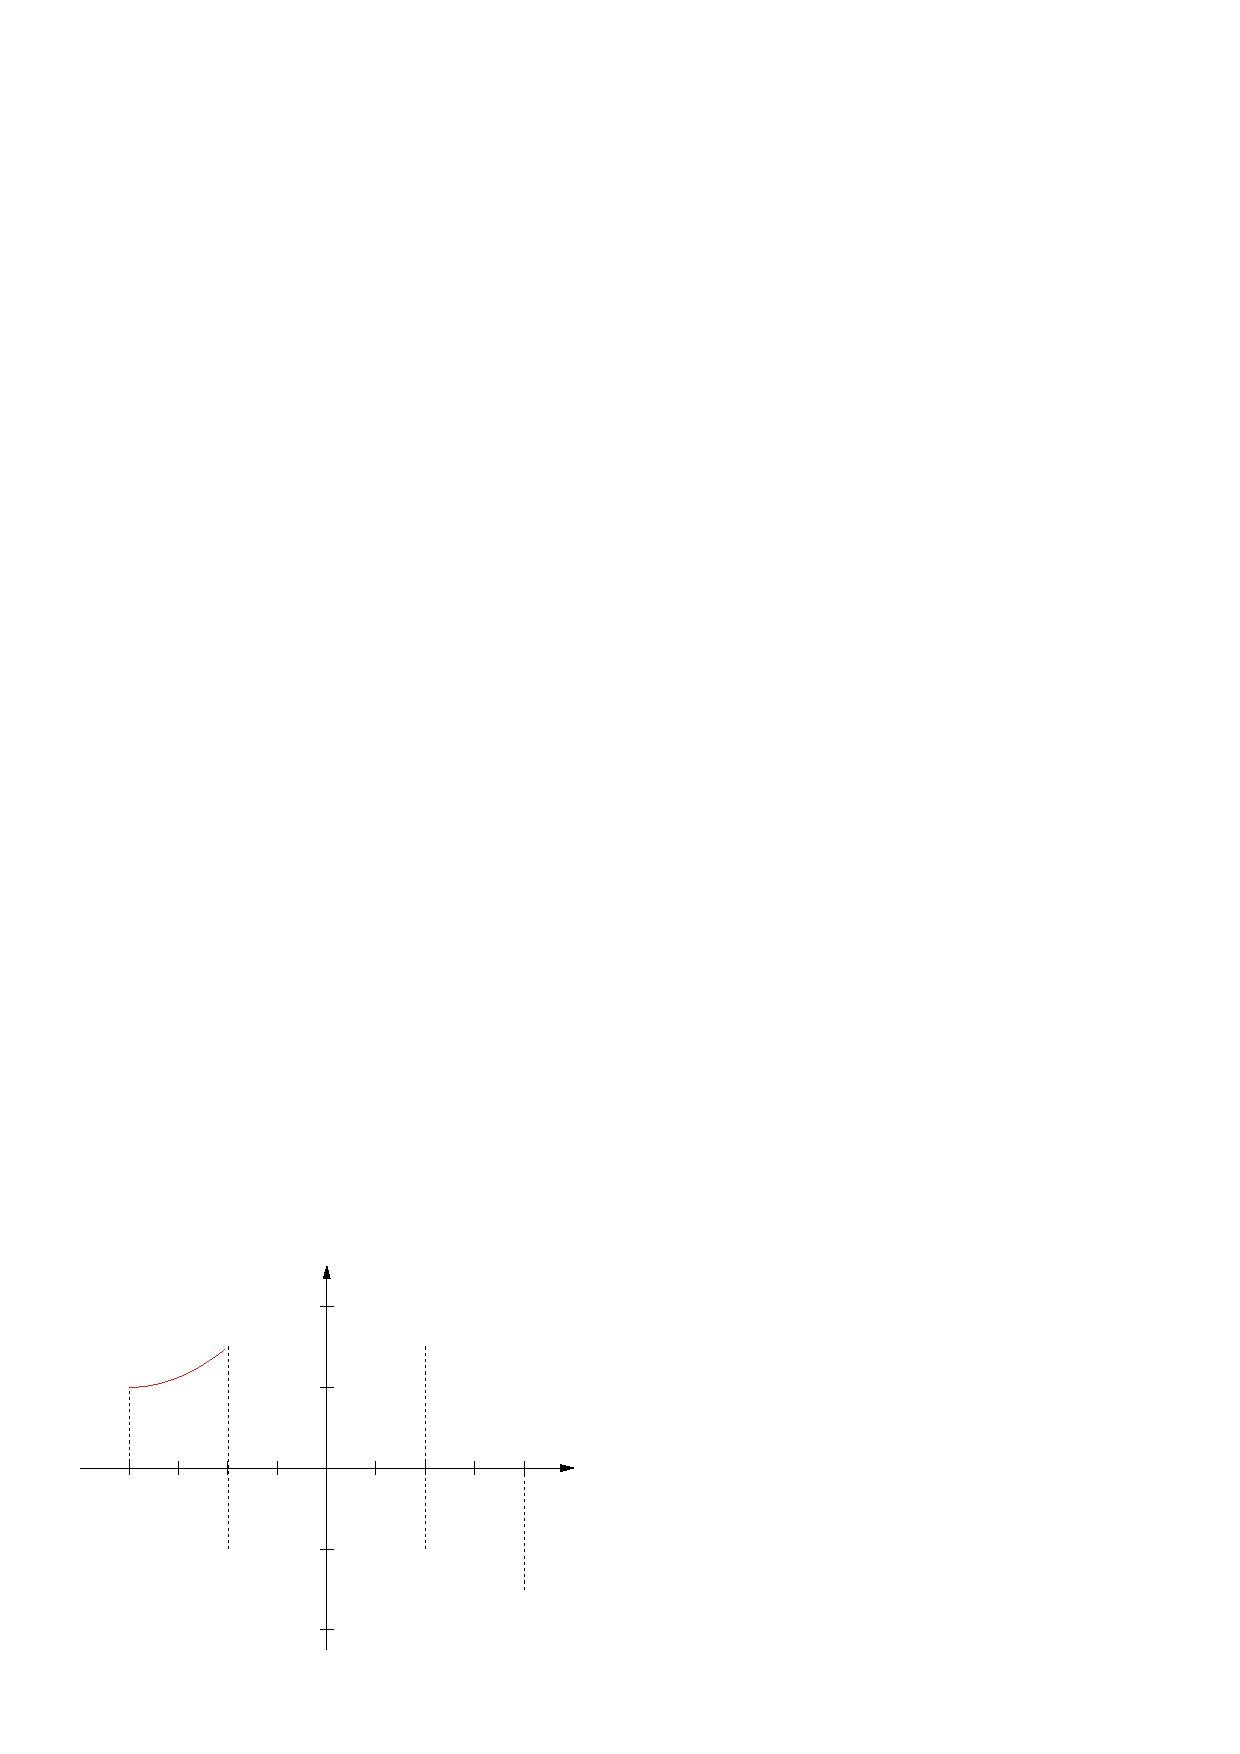
\includegraphics[width={216.00bp},height={172.80bp}]{figura_02_06}}%
    \gplfronttext
  \end{picture}%
\endgroup

    \caption{La gráfica se desplaza $1/2$ periodo\\
    y se refleja respecto a $t$.}
\end{figure}

\subsection{Evaluación de coeficientes de \emph{Fourier}}
\begin{equation*}
\begin{split}
    a_0
        &=\frac{2}{T}\int_0^T f(t)\,dt\\
        &=\frac{2}{T}\left[\int_0^{T/2} f(t)\,dt+\int_{T/2}^T f(t)\,dt\right]\\
        &=\frac{2}{T}\left[
            \int_0^{T/2} f(t)\,dt-\int_{t=T/2}^{t=T} f(t-\frac{T}{2})\,dt
        \right]\\
\end{split}
\end{equation*}
\begin{equation*}
    \tau=t-\frac{T}{2}
\end{equation*}
\begin{equation*}
    d\tau=dt
\end{equation*}
\begin{equation*}
\begin{split}
    a_0
        &=\frac{2}{T}\left[
            \int_0^{T/2} f(t)\,dt-
            \int_{\tau=T/2-T/2}^{\tau=T-T/2} f(\tau)\,d\tau
        \right]\\
        &=\frac{2}{T}\left[
            \int_0^{T/2} f(t)\,dt-\int_0^{T/2} f(\tau)\,d\tau
        \right]\\
\end{split}
\end{equation*}
\begin{equation}
    a_0=0
\end{equation}
\begin{equation*}
\begin{split}
    a_n
        &=\frac{2}{T}\int_0^T f(t)\cos(n\omega_0 t)\,dt\\
        &=\frac{2}{T}\left[
            \int_0^{T/2} f(t)\cos(n\omega_0 t)\,dt+
            \int_{T/2}^T f(t)\cos(n\omega_0 t)\,dt
        \right]\\
        &=\frac{2}{T}\left[
            \int_0^{T/2} f(t)\cos(n\omega_0 t)\,dt-
            \int_{T/2}^T f(t-\frac{T}{2})\cos(n\omega_0 t)\,dt
        \right]\\
\end{split}
\end{equation*}
\begin{equation*}
    \tau=t-\frac{T}{2}
\end{equation*}
\begin{equation*}
    d\tau=dt
\end{equation*}
\begin{equation*}
\begin{split}
    a_n
        &=\frac{2}{T}\left[
            \int_0^{T/2} f(t)\cos(n\omega_0 t)\,dt-
            \int_{\tau=T/2-T/2}^{\tau=T-T/2}
                f(\tau)\cos(n\omega_0(\tau+\frac{T}{2}))\,d\tau
        \right]\\
        &=\frac{2}{T}\left[
            \int_0^{T/2} f(t)\cos(n\omega_0 t)\,dt-
            \int_0^{T/2} f(\tau)\cos(n\omega_0(\tau+\frac{T}{2}))\,d\tau
        \right]\\
\end{split}
\end{equation*}
\begin{equation*}
\begin{split}
    n\omega_0(\tau+T/2)
        &=n\omega_0\tau+n\omega_0\frac{T}{2}\\
        &=n\omega_0\tau+n\frac{2\pi}{T}\frac{T}{2}\\
        &=n\omega_0\tau+n\pi\\
\end{split}
\end{equation*}
\begin{equation*}
\begin{split}
    \cos(n\omega_0\tau+n\pi)
        &=\cos(n\omega_0\tau)\cos(n\pi)-\sen(n\pi)\sen(n\omega_0\tau)\\
        &=\cos(n\omega_0\tau)\cos(n\pi)\\
\end{split}
\end{equation*}
\begin{equation*}
\begin{split}
    a_n
        &=\frac{2}{T}\left[
            \int_0^{T/2} f(t)\cos(n\omega_0 t)\,dt-
            \int_0^{T/2} f(\tau)\cos(n\omega_0\tau)\cos(n\pi)\,d\tau
        \right]\\
        &=\frac{2}{T}\left[
            \int_0^{T/2} f(t)\cos(n\omega_0 t)\,dt-\cos(n\pi)\int_0^{T/2}
                f(\tau)\cos(n\omega_0\tau)\,d\tau
        \right]\\
        &=\frac{2}{T}(1-\cos(\pi n))\left(
            \int_0^{T/2} f(t)\cos(n\omega_0 t)\,dt
        \right)\\
\end{split}
\end{equation*}
\begin{equation*}
    \cos(\pi n)=\begin{cases}
        1 &n: \text{par}\\
        -1 &n: \text{impar}\\
    \end{cases}
\end{equation*}
\begin{equation}
\begin{cases}
    n: \text{par}   &a_n=0\\
    n: \text{impar} &a_n=\frac{4}{T}\int_0^{T/2}f(t)\cos(n\omega_0 t)\,dt\\
\end{cases}
\end{equation}
\begin{equation*}
\begin{split}
    b_n
        &=\frac{2}{T}\int_0^T f(t)\sen(n\omega_0 t)\,dt\\
        &=\frac{2}{T}\left[
            \int_0^{T/2} f(t)\sen(n\omega_0 t)\,dt+
            \int_{T/2}^T f(t)\sen(n\omega_0 t)\,dt
        \right]\\
        &=\frac{2}{T}\left[
            \int_0^{T/2} f(t)\sen(n\omega_0 t)\,dt-
            \int_{T/2}^T f(t-\frac{T}{2})\sen(n\omega_0 t)\,dt
        \right]\\
\end{split}
\end{equation*}
\begin{equation*}
    \tau=t-\frac{T}{2}
\end{equation*}
\begin{equation*}
    d\tau=dt
\end{equation*}
\begin{equation*}
\begin{split}
    b_n
        &=\frac{2}{T}\left[
            \int_0^{T/2} f(t)\sen(n\omega_0 t)\,dt-
            \int_{\tau=T/2-T/2}^{\tau=T-T/2}
                f(\tau)\sen(n\omega_0(\tau+\frac{T}{2}))\,d\tau
        \right]\\
        &=\frac{2}{T}\left[
            \int_0^{T/2} f(t)\sen(n\omega_0 t)\,dt-
            \int_0^{T/2} f(\tau)\sen(n\omega_0(\tau+\frac{T}{2}))\,d\tau
        \right]\\
\end{split}
\end{equation*}
\begin{equation*}
\begin{split}
    n\omega_0(\tau+T/2)
        &=n\omega_0\tau+n\omega_0\frac{T}{2}\\
        &=n\omega_0\tau+n\frac{2\pi}{T}\frac{T}{2}\\
        &=n\omega_0\tau+n\pi\\
\end{split}
\end{equation*}
\begin{equation*}
\begin{split}
    \sen(n\omega_0\tau+n\pi)
        &=\sen(n\omega_0\tau)\cos(n\pi)+\sen(n\pi)\cos(n\omega_0\tau)\\
        &=\sen(n\omega_0\tau)\cos(n\pi)\\
\end{split}
\end{equation*}
\begin{equation*}
\begin{split}
    b_n
        &=\frac{2}{T}\left[
            \int_0^{T/2} f(t)\sen(n\omega_0 t)\,dt-
            \int_0^{T/2} f(\tau)\sen(n\omega_0\tau)\cos(n\pi)\,d\tau
        \right]\\
        &=\frac{2}{T}\left[
            \int_0^{T/2} f(t)\sen(n\omega_0 t)\,dt-
            \cos(n\pi)\int_0^{T/2} f(\tau)\sen(n\omega_0\tau)\,d\tau
        \right]\\
        &=\frac{2}{T}(1-\cos(\pi n))\left(
            \int_0^{T/2} f(t)\sen(n\omega_0 t)\,dt
        \right)\\
\end{split}
\end{equation*}
\begin{equation*}
    \cos(\pi n)=\begin{cases}
        1 &n: \text{par}\\
        -1 &n: \text{impar}\\
    \end{cases}
\end{equation*}
\begin{equation}
\begin{cases}
    n: \text{par}   &b_n=0\\
    n: \text{impar} &b_n=\frac{4}{T}\int_0^{T/2}f(t)\sen(n\omega_0 t)\,dt\\
\end{cases}
\end{equation}

\section{Simetría de cuarto de onda (S.C.O.)}
\subsection{Simetría de cuarto de onda par}
Una función $f(t)$ tiene simetría de cuarto de onda \textbf{par} cuando:
\begin{itemize}
    \item $f(t)$ es \textbf{par}.
    \item $f(t)$ tiene simetría de media onda.
\end{itemize}
\begin{figure}[H]
    \centering
    % GNUPLOT: LaTeX picture with Postscript
\begingroup
  \makeatletter
  \providecommand\color[2][]{%
    \GenericError{(gnuplot) \space\space\space\@spaces}{%
      Package color not loaded in conjunction with
      terminal option `colourtext'%
    }{See the gnuplot documentation for explanation.%
    }{Either use 'blacktext' in gnuplot or load the package
      color.sty in LaTeX.}%
    \renewcommand\color[2][]{}%
  }%
  \providecommand\includegraphics[2][]{%
    \GenericError{(gnuplot) \space\space\space\@spaces}{%
      Package graphicx or graphics not loaded%
    }{See the gnuplot documentation for explanation.%
    }{The gnuplot epslatex terminal needs graphicx.sty or graphics.sty.}%
    \renewcommand\includegraphics[2][]{}%
  }%
  \providecommand\rotatebox[2]{#2}%
  \@ifundefined{ifGPcolor}{%
    \newif\ifGPcolor
    \GPcolorfalse
  }{}%
  \@ifundefined{ifGPblacktext}{%
    \newif\ifGPblacktext
    \GPblacktexttrue
  }{}%
  % define a \g@addto@macro without @ in the name:
  \let\gplgaddtomacro\g@addto@macro
  % define empty templates for all commands taking text:
  \gdef\gplbacktext{}%
  \gdef\gplfronttext{}%
  \makeatother
  \ifGPblacktext
    % no textcolor at all
    \def\colorrgb#1{}%
    \def\colorgray#1{}%
  \else
    % gray or color?
    \ifGPcolor
      \def\colorrgb#1{\color[rgb]{#1}}%
      \def\colorgray#1{\color[gray]{#1}}%
      \expandafter\def\csname LTw\endcsname{\color{white}}%
      \expandafter\def\csname LTb\endcsname{\color{black}}%
      \expandafter\def\csname LTa\endcsname{\color{black}}%
      \expandafter\def\csname LT0\endcsname{\color[rgb]{1,0,0}}%
      \expandafter\def\csname LT1\endcsname{\color[rgb]{0,1,0}}%
      \expandafter\def\csname LT2\endcsname{\color[rgb]{0,0,1}}%
      \expandafter\def\csname LT3\endcsname{\color[rgb]{1,0,1}}%
      \expandafter\def\csname LT4\endcsname{\color[rgb]{0,1,1}}%
      \expandafter\def\csname LT5\endcsname{\color[rgb]{1,1,0}}%
      \expandafter\def\csname LT6\endcsname{\color[rgb]{0,0,0}}%
      \expandafter\def\csname LT7\endcsname{\color[rgb]{1,0.3,0}}%
      \expandafter\def\csname LT8\endcsname{\color[rgb]{0.5,0.5,0.5}}%
    \else
      % gray
      \def\colorrgb#1{\color{black}}%
      \def\colorgray#1{\color[gray]{#1}}%
      \expandafter\def\csname LTw\endcsname{\color{white}}%
      \expandafter\def\csname LTb\endcsname{\color{black}}%
      \expandafter\def\csname LTa\endcsname{\color{black}}%
      \expandafter\def\csname LT0\endcsname{\color{black}}%
      \expandafter\def\csname LT1\endcsname{\color{black}}%
      \expandafter\def\csname LT2\endcsname{\color{black}}%
      \expandafter\def\csname LT3\endcsname{\color{black}}%
      \expandafter\def\csname LT4\endcsname{\color{black}}%
      \expandafter\def\csname LT5\endcsname{\color{black}}%
      \expandafter\def\csname LT6\endcsname{\color{black}}%
      \expandafter\def\csname LT7\endcsname{\color{black}}%
      \expandafter\def\csname LT8\endcsname{\color{black}}%
    \fi
  \fi
    \setlength{\unitlength}{0.0500bp}%
    \ifx\gptboxheight\undefined%
      \newlength{\gptboxheight}%
      \newlength{\gptboxwidth}%
      \newsavebox{\gptboxtext}%
    \fi%
    \setlength{\fboxrule}{0.5pt}%
    \setlength{\fboxsep}{1pt}%
    \definecolor{tbcol}{rgb}{1,1,1}%
\begin{picture}(7200.00,3456.00)%
    \gplgaddtomacro\gplbacktext{%
      \csname LTb\endcsname%%
      \put(3480,192){\makebox(0,0)[r]{\strut{}}}%
      \put(3480,709){\makebox(0,0)[r]{\strut{}}}%
      \put(3480,1226){\makebox(0,0)[r]{\strut{}}}%
      \put(3480,1744){\makebox(0,0)[r]{\strut{}}}%
      \put(3480,2261){\makebox(0,0)[r]{\strut{}}}%
      \put(3480,2778){\makebox(0,0)[r]{\strut{}}}%
      \put(3480,3295){\makebox(0,0)[r]{\strut{}}}%
      \put(240,1521){\makebox(0,0){\strut{}}}%
      \put(907,1521){\makebox(0,0){\strut{}}}%
      \put(1574,1521){\makebox(0,0){\strut{}}}%
      \put(2241,1521){\makebox(0,0){\strut{}}}%
      \put(2908,1521){\makebox(0,0){\strut{}}}%
      \put(3576,1521){\makebox(0,0){\strut{}}}%
      \put(4243,1521){\makebox(0,0){\strut{}}}%
      \put(4910,1521){\makebox(0,0){\strut{}}}%
      \put(5577,1521){\makebox(0,0){\strut{}}}%
      \put(6244,1521){\makebox(0,0){\strut{}}}%
      \put(6911,1521){\makebox(0,0){\strut{}}}%
      \csname LTb\endcsname%%
      \put(7778,1744){\makebox(0,0)[l]{\strut{}$t$}}%
      \put(3876,3502){\makebox(0,0)[l]{\strut{}$f(t)$}}%
      \put(640,1485){\makebox(0,0)[l]{\strut{}$-T$}}%
      \put(1307,1485){\makebox(0,0)[l]{\strut{}$-\frac{3T}{4}$}}%
      \put(1974,1485){\makebox(0,0)[l]{\strut{}$-\frac{T}{2}$}}%
      \put(2642,1485){\makebox(0,0)[l]{\strut{}$-\frac{T}{4}$}}%
      \put(4176,1485){\makebox(0,0)[l]{\strut{}$ \frac{T}{4}$}}%
      \put(4776,1485){\makebox(0,0)[l]{\strut{}$ \frac{T}{2}$}}%
      \put(5443,1485){\makebox(0,0)[l]{\strut{}$ \frac{3T}{4}$}}%
      \put(6177,1485){\makebox(0,0)[l]{\strut{}$T$}}%
    }%
    \gplgaddtomacro\gplfronttext{%
    }%
    \gplgaddtomacro\gplbacktext{%
      \csname LTb\endcsname%%
      \put(3480,192){\makebox(0,0)[r]{\strut{}}}%
      \put(3480,709){\makebox(0,0)[r]{\strut{}}}%
      \put(3480,1226){\makebox(0,0)[r]{\strut{}}}%
      \put(3480,1744){\makebox(0,0)[r]{\strut{}}}%
      \put(3480,2261){\makebox(0,0)[r]{\strut{}}}%
      \put(3480,2778){\makebox(0,0)[r]{\strut{}}}%
      \put(3480,3295){\makebox(0,0)[r]{\strut{}}}%
      \put(240,1521){\makebox(0,0){\strut{}}}%
      \put(907,1521){\makebox(0,0){\strut{}}}%
      \put(1574,1521){\makebox(0,0){\strut{}}}%
      \put(2241,1521){\makebox(0,0){\strut{}}}%
      \put(2908,1521){\makebox(0,0){\strut{}}}%
      \put(3576,1521){\makebox(0,0){\strut{}}}%
      \put(4243,1521){\makebox(0,0){\strut{}}}%
      \put(4910,1521){\makebox(0,0){\strut{}}}%
      \put(5577,1521){\makebox(0,0){\strut{}}}%
      \put(6244,1521){\makebox(0,0){\strut{}}}%
      \put(6911,1521){\makebox(0,0){\strut{}}}%
      \csname LTb\endcsname%%
      \put(7778,1744){\makebox(0,0)[l]{\strut{}$t$}}%
      \put(3876,3502){\makebox(0,0)[l]{\strut{}$f(t)$}}%
      \put(640,1485){\makebox(0,0)[l]{\strut{}$-T$}}%
      \put(1307,1485){\makebox(0,0)[l]{\strut{}$-\frac{3T}{4}$}}%
      \put(1974,1485){\makebox(0,0)[l]{\strut{}$-\frac{T}{2}$}}%
      \put(2642,1485){\makebox(0,0)[l]{\strut{}$-\frac{T}{4}$}}%
      \put(4176,1485){\makebox(0,0)[l]{\strut{}$ \frac{T}{4}$}}%
      \put(4776,1485){\makebox(0,0)[l]{\strut{}$ \frac{T}{2}$}}%
      \put(5443,1485){\makebox(0,0)[l]{\strut{}$ \frac{3T}{4}$}}%
      \put(6177,1485){\makebox(0,0)[l]{\strut{}$T$}}%
    }%
    \gplgaddtomacro\gplfronttext{%
    }%
    \gplgaddtomacro\gplbacktext{%
      \csname LTb\endcsname%%
      \put(3480,192){\makebox(0,0)[r]{\strut{}}}%
      \put(3480,709){\makebox(0,0)[r]{\strut{}}}%
      \put(3480,1226){\makebox(0,0)[r]{\strut{}}}%
      \put(3480,1744){\makebox(0,0)[r]{\strut{}}}%
      \put(3480,2261){\makebox(0,0)[r]{\strut{}}}%
      \put(3480,2778){\makebox(0,0)[r]{\strut{}}}%
      \put(3480,3295){\makebox(0,0)[r]{\strut{}}}%
      \put(240,1521){\makebox(0,0){\strut{}}}%
      \put(907,1521){\makebox(0,0){\strut{}}}%
      \put(1574,1521){\makebox(0,0){\strut{}}}%
      \put(2241,1521){\makebox(0,0){\strut{}}}%
      \put(2908,1521){\makebox(0,0){\strut{}}}%
      \put(3576,1521){\makebox(0,0){\strut{}}}%
      \put(4243,1521){\makebox(0,0){\strut{}}}%
      \put(4910,1521){\makebox(0,0){\strut{}}}%
      \put(5577,1521){\makebox(0,0){\strut{}}}%
      \put(6244,1521){\makebox(0,0){\strut{}}}%
      \put(6911,1521){\makebox(0,0){\strut{}}}%
      \csname LTb\endcsname%%
      \put(7778,1744){\makebox(0,0)[l]{\strut{}$t$}}%
      \put(3876,3502){\makebox(0,0)[l]{\strut{}$f(t)$}}%
      \put(640,1485){\makebox(0,0)[l]{\strut{}$-T$}}%
      \put(1307,1485){\makebox(0,0)[l]{\strut{}$-\frac{3T}{4}$}}%
      \put(1974,1485){\makebox(0,0)[l]{\strut{}$-\frac{T}{2}$}}%
      \put(2642,1485){\makebox(0,0)[l]{\strut{}$-\frac{T}{4}$}}%
      \put(4176,1485){\makebox(0,0)[l]{\strut{}$ \frac{T}{4}$}}%
      \put(4776,1485){\makebox(0,0)[l]{\strut{}$ \frac{T}{2}$}}%
      \put(5443,1485){\makebox(0,0)[l]{\strut{}$ \frac{3T}{4}$}}%
      \put(6177,1485){\makebox(0,0)[l]{\strut{}$T$}}%
    }%
    \gplgaddtomacro\gplfronttext{%
    }%
    \gplgaddtomacro\gplbacktext{%
      \csname LTb\endcsname%%
      \put(3480,192){\makebox(0,0)[r]{\strut{}}}%
      \put(3480,709){\makebox(0,0)[r]{\strut{}}}%
      \put(3480,1226){\makebox(0,0)[r]{\strut{}}}%
      \put(3480,1744){\makebox(0,0)[r]{\strut{}}}%
      \put(3480,2261){\makebox(0,0)[r]{\strut{}}}%
      \put(3480,2778){\makebox(0,0)[r]{\strut{}}}%
      \put(3480,3295){\makebox(0,0)[r]{\strut{}}}%
      \put(240,1521){\makebox(0,0){\strut{}}}%
      \put(907,1521){\makebox(0,0){\strut{}}}%
      \put(1574,1521){\makebox(0,0){\strut{}}}%
      \put(2241,1521){\makebox(0,0){\strut{}}}%
      \put(2908,1521){\makebox(0,0){\strut{}}}%
      \put(3576,1521){\makebox(0,0){\strut{}}}%
      \put(4243,1521){\makebox(0,0){\strut{}}}%
      \put(4910,1521){\makebox(0,0){\strut{}}}%
      \put(5577,1521){\makebox(0,0){\strut{}}}%
      \put(6244,1521){\makebox(0,0){\strut{}}}%
      \put(6911,1521){\makebox(0,0){\strut{}}}%
      \csname LTb\endcsname%%
      \put(7778,1744){\makebox(0,0)[l]{\strut{}$t$}}%
      \put(3876,3502){\makebox(0,0)[l]{\strut{}$f(t)$}}%
      \put(640,1485){\makebox(0,0)[l]{\strut{}$-T$}}%
      \put(1307,1485){\makebox(0,0)[l]{\strut{}$-\frac{3T}{4}$}}%
      \put(1974,1485){\makebox(0,0)[l]{\strut{}$-\frac{T}{2}$}}%
      \put(2642,1485){\makebox(0,0)[l]{\strut{}$-\frac{T}{4}$}}%
      \put(4176,1485){\makebox(0,0)[l]{\strut{}$ \frac{T}{4}$}}%
      \put(4776,1485){\makebox(0,0)[l]{\strut{}$ \frac{T}{2}$}}%
      \put(5443,1485){\makebox(0,0)[l]{\strut{}$ \frac{3T}{4}$}}%
      \put(6177,1485){\makebox(0,0)[l]{\strut{}$T$}}%
    }%
    \gplgaddtomacro\gplfronttext{%
    }%
    \gplgaddtomacro\gplbacktext{%
      \csname LTb\endcsname%%
      \put(3480,192){\makebox(0,0)[r]{\strut{}}}%
      \put(3480,709){\makebox(0,0)[r]{\strut{}}}%
      \put(3480,1226){\makebox(0,0)[r]{\strut{}}}%
      \put(3480,1744){\makebox(0,0)[r]{\strut{}}}%
      \put(3480,2261){\makebox(0,0)[r]{\strut{}}}%
      \put(3480,2778){\makebox(0,0)[r]{\strut{}}}%
      \put(3480,3295){\makebox(0,0)[r]{\strut{}}}%
      \put(240,1521){\makebox(0,0){\strut{}}}%
      \put(907,1521){\makebox(0,0){\strut{}}}%
      \put(1574,1521){\makebox(0,0){\strut{}}}%
      \put(2241,1521){\makebox(0,0){\strut{}}}%
      \put(2908,1521){\makebox(0,0){\strut{}}}%
      \put(3576,1521){\makebox(0,0){\strut{}}}%
      \put(4243,1521){\makebox(0,0){\strut{}}}%
      \put(4910,1521){\makebox(0,0){\strut{}}}%
      \put(5577,1521){\makebox(0,0){\strut{}}}%
      \put(6244,1521){\makebox(0,0){\strut{}}}%
      \put(6911,1521){\makebox(0,0){\strut{}}}%
      \csname LTb\endcsname%%
      \put(7778,1744){\makebox(0,0)[l]{\strut{}$t$}}%
      \put(3876,3502){\makebox(0,0)[l]{\strut{}$f(t)$}}%
      \put(640,1485){\makebox(0,0)[l]{\strut{}$-T$}}%
      \put(1307,1485){\makebox(0,0)[l]{\strut{}$-\frac{3T}{4}$}}%
      \put(1974,1485){\makebox(0,0)[l]{\strut{}$-\frac{T}{2}$}}%
      \put(2642,1485){\makebox(0,0)[l]{\strut{}$-\frac{T}{4}$}}%
      \put(4176,1485){\makebox(0,0)[l]{\strut{}$ \frac{T}{4}$}}%
      \put(4776,1485){\makebox(0,0)[l]{\strut{}$ \frac{T}{2}$}}%
      \put(5443,1485){\makebox(0,0)[l]{\strut{}$ \frac{3T}{4}$}}%
      \put(6177,1485){\makebox(0,0)[l]{\strut{}$T$}}%
    }%
    \gplgaddtomacro\gplfronttext{%
    }%
    \gplbacktext
    \put(0,0){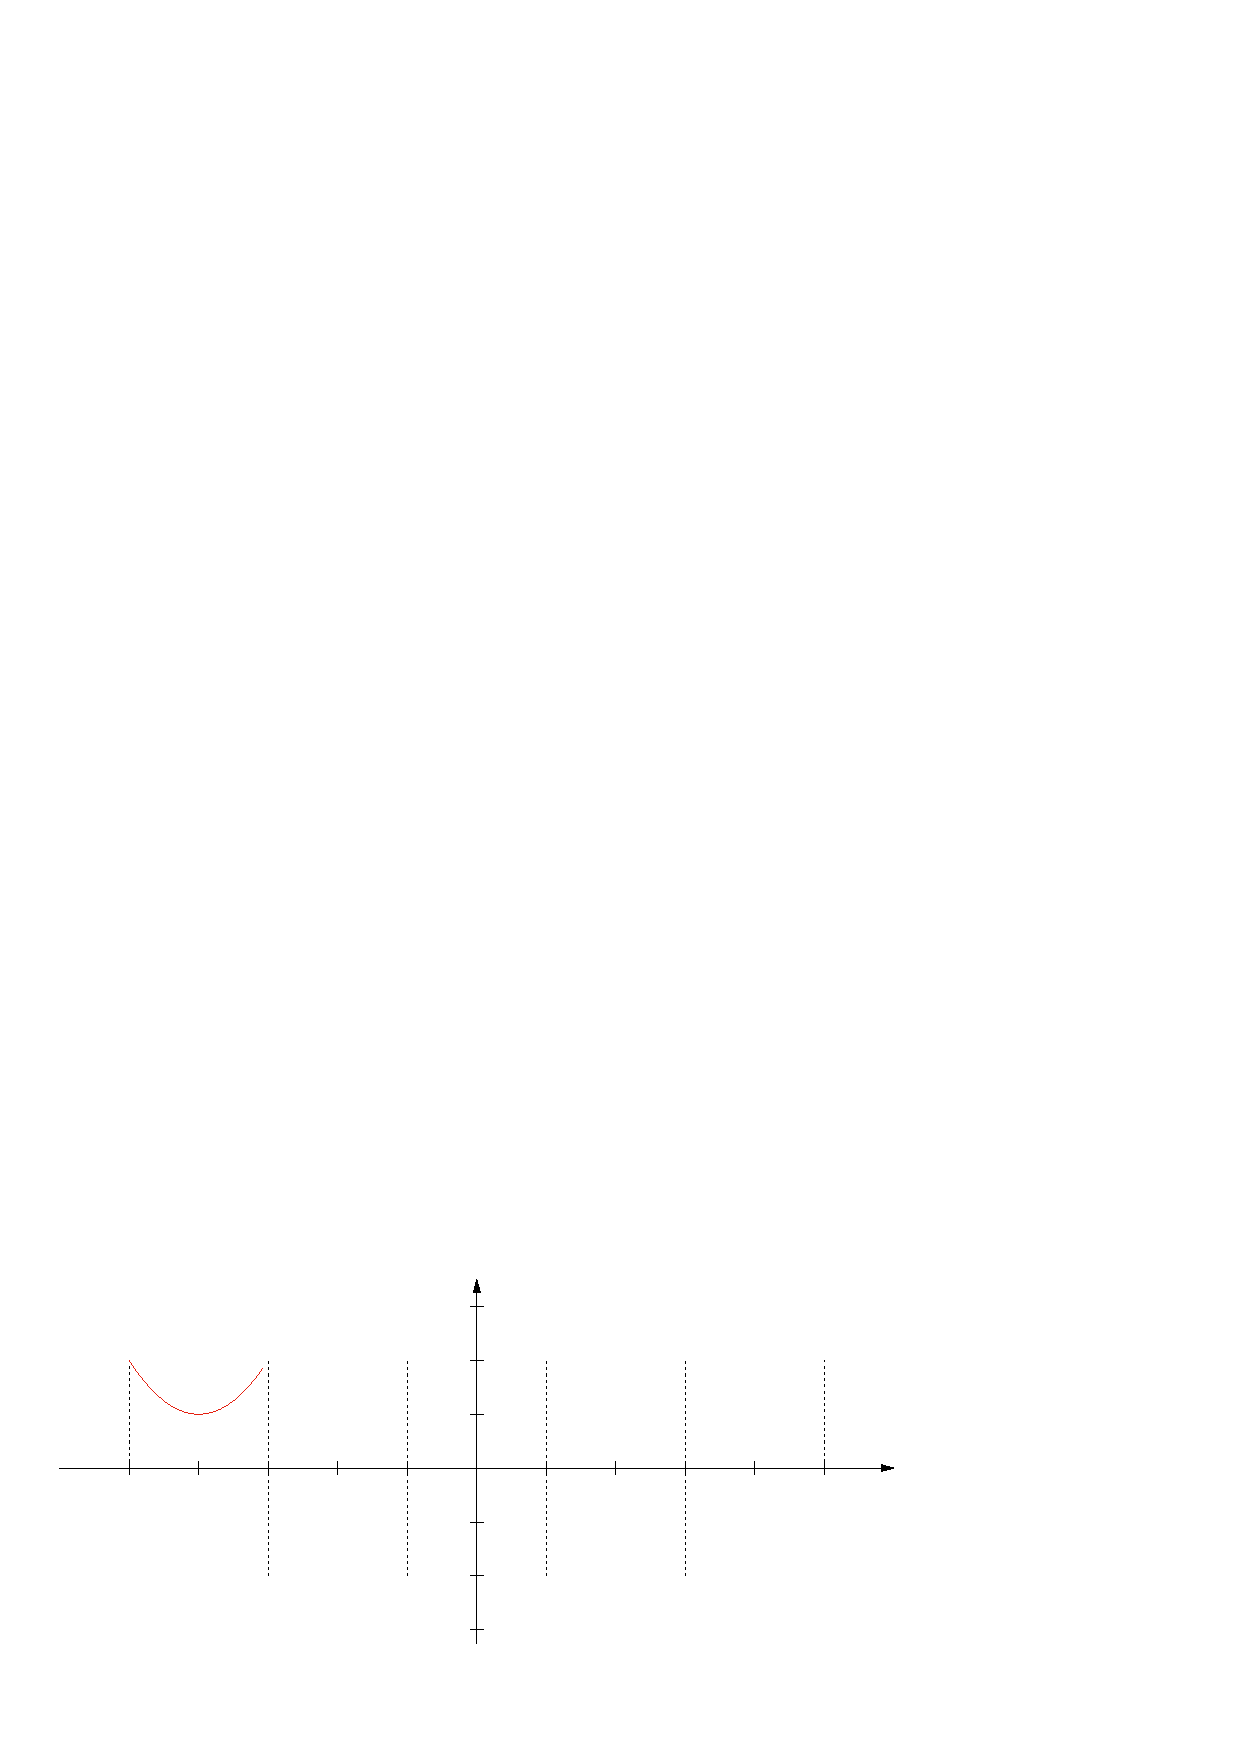
\includegraphics[width={360.00bp},height={172.80bp}]{figura_02_07}}%
    \gplfronttext
  \end{picture}%
\endgroup

\end{figure}

\subsection{Simetría de cuarto de onda impar}
Una función $f(t)$ tiene simetría de cuarto de onda \textbf{impar} cuando:
\begin{itemize}
    \item $f(t)$ es \textbf{impar}.
    \item $f(t)$ tiene simetría de media onda.
\end{itemize}
\begin{figure}[H]
    \centering
    % GNUPLOT: LaTeX picture with Postscript
\begingroup
  \makeatletter
  \providecommand\color[2][]{%
    \GenericError{(gnuplot) \space\space\space\@spaces}{%
      Package color not loaded in conjunction with
      terminal option `colourtext'%
    }{See the gnuplot documentation for explanation.%
    }{Either use 'blacktext' in gnuplot or load the package
      color.sty in LaTeX.}%
    \renewcommand\color[2][]{}%
  }%
  \providecommand\includegraphics[2][]{%
    \GenericError{(gnuplot) \space\space\space\@spaces}{%
      Package graphicx or graphics not loaded%
    }{See the gnuplot documentation for explanation.%
    }{The gnuplot epslatex terminal needs graphicx.sty or graphics.sty.}%
    \renewcommand\includegraphics[2][]{}%
  }%
  \providecommand\rotatebox[2]{#2}%
  \@ifundefined{ifGPcolor}{%
    \newif\ifGPcolor
    \GPcolorfalse
  }{}%
  \@ifundefined{ifGPblacktext}{%
    \newif\ifGPblacktext
    \GPblacktexttrue
  }{}%
  % define a \g@addto@macro without @ in the name:
  \let\gplgaddtomacro\g@addto@macro
  % define empty templates for all commands taking text:
  \gdef\gplbacktext{}%
  \gdef\gplfronttext{}%
  \makeatother
  \ifGPblacktext
    % no textcolor at all
    \def\colorrgb#1{}%
    \def\colorgray#1{}%
  \else
    % gray or color?
    \ifGPcolor
      \def\colorrgb#1{\color[rgb]{#1}}%
      \def\colorgray#1{\color[gray]{#1}}%
      \expandafter\def\csname LTw\endcsname{\color{white}}%
      \expandafter\def\csname LTb\endcsname{\color{black}}%
      \expandafter\def\csname LTa\endcsname{\color{black}}%
      \expandafter\def\csname LT0\endcsname{\color[rgb]{1,0,0}}%
      \expandafter\def\csname LT1\endcsname{\color[rgb]{0,1,0}}%
      \expandafter\def\csname LT2\endcsname{\color[rgb]{0,0,1}}%
      \expandafter\def\csname LT3\endcsname{\color[rgb]{1,0,1}}%
      \expandafter\def\csname LT4\endcsname{\color[rgb]{0,1,1}}%
      \expandafter\def\csname LT5\endcsname{\color[rgb]{1,1,0}}%
      \expandafter\def\csname LT6\endcsname{\color[rgb]{0,0,0}}%
      \expandafter\def\csname LT7\endcsname{\color[rgb]{1,0.3,0}}%
      \expandafter\def\csname LT8\endcsname{\color[rgb]{0.5,0.5,0.5}}%
    \else
      % gray
      \def\colorrgb#1{\color{black}}%
      \def\colorgray#1{\color[gray]{#1}}%
      \expandafter\def\csname LTw\endcsname{\color{white}}%
      \expandafter\def\csname LTb\endcsname{\color{black}}%
      \expandafter\def\csname LTa\endcsname{\color{black}}%
      \expandafter\def\csname LT0\endcsname{\color{black}}%
      \expandafter\def\csname LT1\endcsname{\color{black}}%
      \expandafter\def\csname LT2\endcsname{\color{black}}%
      \expandafter\def\csname LT3\endcsname{\color{black}}%
      \expandafter\def\csname LT4\endcsname{\color{black}}%
      \expandafter\def\csname LT5\endcsname{\color{black}}%
      \expandafter\def\csname LT6\endcsname{\color{black}}%
      \expandafter\def\csname LT7\endcsname{\color{black}}%
      \expandafter\def\csname LT8\endcsname{\color{black}}%
    \fi
  \fi
    \setlength{\unitlength}{0.0500bp}%
    \ifx\gptboxheight\undefined%
      \newlength{\gptboxheight}%
      \newlength{\gptboxwidth}%
      \newsavebox{\gptboxtext}%
    \fi%
    \setlength{\fboxrule}{0.5pt}%
    \setlength{\fboxsep}{1pt}%
    \definecolor{tbcol}{rgb}{1,1,1}%
\begin{picture}(7200.00,3456.00)%
    \gplgaddtomacro\gplbacktext{%
      \csname LTb\endcsname%%
      \put(3480,192){\makebox(0,0)[r]{\strut{}}}%
      \put(3480,709){\makebox(0,0)[r]{\strut{}}}%
      \put(3480,1226){\makebox(0,0)[r]{\strut{}}}%
      \put(3480,1744){\makebox(0,0)[r]{\strut{}}}%
      \put(3480,2261){\makebox(0,0)[r]{\strut{}}}%
      \put(3480,2778){\makebox(0,0)[r]{\strut{}}}%
      \put(3480,3295){\makebox(0,0)[r]{\strut{}}}%
      \put(240,1521){\makebox(0,0){\strut{}}}%
      \put(907,1521){\makebox(0,0){\strut{}}}%
      \put(1574,1521){\makebox(0,0){\strut{}}}%
      \put(2241,1521){\makebox(0,0){\strut{}}}%
      \put(2908,1521){\makebox(0,0){\strut{}}}%
      \put(3576,1521){\makebox(0,0){\strut{}}}%
      \put(4243,1521){\makebox(0,0){\strut{}}}%
      \put(4910,1521){\makebox(0,0){\strut{}}}%
      \put(5577,1521){\makebox(0,0){\strut{}}}%
      \put(6244,1521){\makebox(0,0){\strut{}}}%
      \put(6911,1521){\makebox(0,0){\strut{}}}%
      \csname LTb\endcsname%%
      \put(7778,1744){\makebox(0,0)[l]{\strut{}$t$}}%
      \put(3876,3502){\makebox(0,0)[l]{\strut{}$f(t)$}}%
      \put(640,1485){\makebox(0,0)[l]{\strut{}$-T$}}%
      \put(1307,1485){\makebox(0,0)[l]{\strut{}$-\frac{3T}{4}$}}%
      \put(1974,1485){\makebox(0,0)[l]{\strut{}$-\frac{T}{2}$}}%
      \put(2642,1485){\makebox(0,0)[l]{\strut{}$-\frac{T}{4}$}}%
      \put(4176,1485){\makebox(0,0)[l]{\strut{}$ \frac{T}{4}$}}%
      \put(4776,1485){\makebox(0,0)[l]{\strut{}$ \frac{T}{2}$}}%
      \put(5443,1485){\makebox(0,0)[l]{\strut{}$ \frac{3T}{4}$}}%
      \put(6177,1485){\makebox(0,0)[l]{\strut{}$T$}}%
    }%
    \gplgaddtomacro\gplfronttext{%
    }%
    \gplgaddtomacro\gplbacktext{%
      \csname LTb\endcsname%%
      \put(3480,192){\makebox(0,0)[r]{\strut{}}}%
      \put(3480,709){\makebox(0,0)[r]{\strut{}}}%
      \put(3480,1226){\makebox(0,0)[r]{\strut{}}}%
      \put(3480,1744){\makebox(0,0)[r]{\strut{}}}%
      \put(3480,2261){\makebox(0,0)[r]{\strut{}}}%
      \put(3480,2778){\makebox(0,0)[r]{\strut{}}}%
      \put(3480,3295){\makebox(0,0)[r]{\strut{}}}%
      \put(240,1521){\makebox(0,0){\strut{}}}%
      \put(907,1521){\makebox(0,0){\strut{}}}%
      \put(1574,1521){\makebox(0,0){\strut{}}}%
      \put(2241,1521){\makebox(0,0){\strut{}}}%
      \put(2908,1521){\makebox(0,0){\strut{}}}%
      \put(3576,1521){\makebox(0,0){\strut{}}}%
      \put(4243,1521){\makebox(0,0){\strut{}}}%
      \put(4910,1521){\makebox(0,0){\strut{}}}%
      \put(5577,1521){\makebox(0,0){\strut{}}}%
      \put(6244,1521){\makebox(0,0){\strut{}}}%
      \put(6911,1521){\makebox(0,0){\strut{}}}%
      \csname LTb\endcsname%%
      \put(7778,1744){\makebox(0,0)[l]{\strut{}$t$}}%
      \put(3876,3502){\makebox(0,0)[l]{\strut{}$f(t)$}}%
      \put(640,1485){\makebox(0,0)[l]{\strut{}$-T$}}%
      \put(1307,1485){\makebox(0,0)[l]{\strut{}$-\frac{3T}{4}$}}%
      \put(1974,1485){\makebox(0,0)[l]{\strut{}$-\frac{T}{2}$}}%
      \put(2642,1485){\makebox(0,0)[l]{\strut{}$-\frac{T}{4}$}}%
      \put(4176,1485){\makebox(0,0)[l]{\strut{}$ \frac{T}{4}$}}%
      \put(4776,1485){\makebox(0,0)[l]{\strut{}$ \frac{T}{2}$}}%
      \put(5443,1485){\makebox(0,0)[l]{\strut{}$ \frac{3T}{4}$}}%
      \put(6177,1485){\makebox(0,0)[l]{\strut{}$T$}}%
    }%
    \gplgaddtomacro\gplfronttext{%
    }%
    \gplgaddtomacro\gplbacktext{%
      \csname LTb\endcsname%%
      \put(3480,192){\makebox(0,0)[r]{\strut{}}}%
      \put(3480,709){\makebox(0,0)[r]{\strut{}}}%
      \put(3480,1226){\makebox(0,0)[r]{\strut{}}}%
      \put(3480,1744){\makebox(0,0)[r]{\strut{}}}%
      \put(3480,2261){\makebox(0,0)[r]{\strut{}}}%
      \put(3480,2778){\makebox(0,0)[r]{\strut{}}}%
      \put(3480,3295){\makebox(0,0)[r]{\strut{}}}%
      \put(240,1521){\makebox(0,0){\strut{}}}%
      \put(907,1521){\makebox(0,0){\strut{}}}%
      \put(1574,1521){\makebox(0,0){\strut{}}}%
      \put(2241,1521){\makebox(0,0){\strut{}}}%
      \put(2908,1521){\makebox(0,0){\strut{}}}%
      \put(3576,1521){\makebox(0,0){\strut{}}}%
      \put(4243,1521){\makebox(0,0){\strut{}}}%
      \put(4910,1521){\makebox(0,0){\strut{}}}%
      \put(5577,1521){\makebox(0,0){\strut{}}}%
      \put(6244,1521){\makebox(0,0){\strut{}}}%
      \put(6911,1521){\makebox(0,0){\strut{}}}%
      \csname LTb\endcsname%%
      \put(7778,1744){\makebox(0,0)[l]{\strut{}$t$}}%
      \put(3876,3502){\makebox(0,0)[l]{\strut{}$f(t)$}}%
      \put(640,1485){\makebox(0,0)[l]{\strut{}$-T$}}%
      \put(1307,1485){\makebox(0,0)[l]{\strut{}$-\frac{3T}{4}$}}%
      \put(1974,1485){\makebox(0,0)[l]{\strut{}$-\frac{T}{2}$}}%
      \put(2642,1485){\makebox(0,0)[l]{\strut{}$-\frac{T}{4}$}}%
      \put(4176,1485){\makebox(0,0)[l]{\strut{}$ \frac{T}{4}$}}%
      \put(4776,1485){\makebox(0,0)[l]{\strut{}$ \frac{T}{2}$}}%
      \put(5443,1485){\makebox(0,0)[l]{\strut{}$ \frac{3T}{4}$}}%
      \put(6177,1485){\makebox(0,0)[l]{\strut{}$T$}}%
    }%
    \gplgaddtomacro\gplfronttext{%
    }%
    \gplgaddtomacro\gplbacktext{%
      \csname LTb\endcsname%%
      \put(3480,192){\makebox(0,0)[r]{\strut{}}}%
      \put(3480,709){\makebox(0,0)[r]{\strut{}}}%
      \put(3480,1226){\makebox(0,0)[r]{\strut{}}}%
      \put(3480,1744){\makebox(0,0)[r]{\strut{}}}%
      \put(3480,2261){\makebox(0,0)[r]{\strut{}}}%
      \put(3480,2778){\makebox(0,0)[r]{\strut{}}}%
      \put(3480,3295){\makebox(0,0)[r]{\strut{}}}%
      \put(240,1521){\makebox(0,0){\strut{}}}%
      \put(907,1521){\makebox(0,0){\strut{}}}%
      \put(1574,1521){\makebox(0,0){\strut{}}}%
      \put(2241,1521){\makebox(0,0){\strut{}}}%
      \put(2908,1521){\makebox(0,0){\strut{}}}%
      \put(3576,1521){\makebox(0,0){\strut{}}}%
      \put(4243,1521){\makebox(0,0){\strut{}}}%
      \put(4910,1521){\makebox(0,0){\strut{}}}%
      \put(5577,1521){\makebox(0,0){\strut{}}}%
      \put(6244,1521){\makebox(0,0){\strut{}}}%
      \put(6911,1521){\makebox(0,0){\strut{}}}%
      \csname LTb\endcsname%%
      \put(7778,1744){\makebox(0,0)[l]{\strut{}$t$}}%
      \put(3876,3502){\makebox(0,0)[l]{\strut{}$f(t)$}}%
      \put(640,1485){\makebox(0,0)[l]{\strut{}$-T$}}%
      \put(1307,1485){\makebox(0,0)[l]{\strut{}$-\frac{3T}{4}$}}%
      \put(1974,1485){\makebox(0,0)[l]{\strut{}$-\frac{T}{2}$}}%
      \put(2642,1485){\makebox(0,0)[l]{\strut{}$-\frac{T}{4}$}}%
      \put(4176,1485){\makebox(0,0)[l]{\strut{}$ \frac{T}{4}$}}%
      \put(4776,1485){\makebox(0,0)[l]{\strut{}$ \frac{T}{2}$}}%
      \put(5443,1485){\makebox(0,0)[l]{\strut{}$ \frac{3T}{4}$}}%
      \put(6177,1485){\makebox(0,0)[l]{\strut{}$T$}}%
    }%
    \gplgaddtomacro\gplfronttext{%
    }%
    \gplbacktext
    \put(0,0){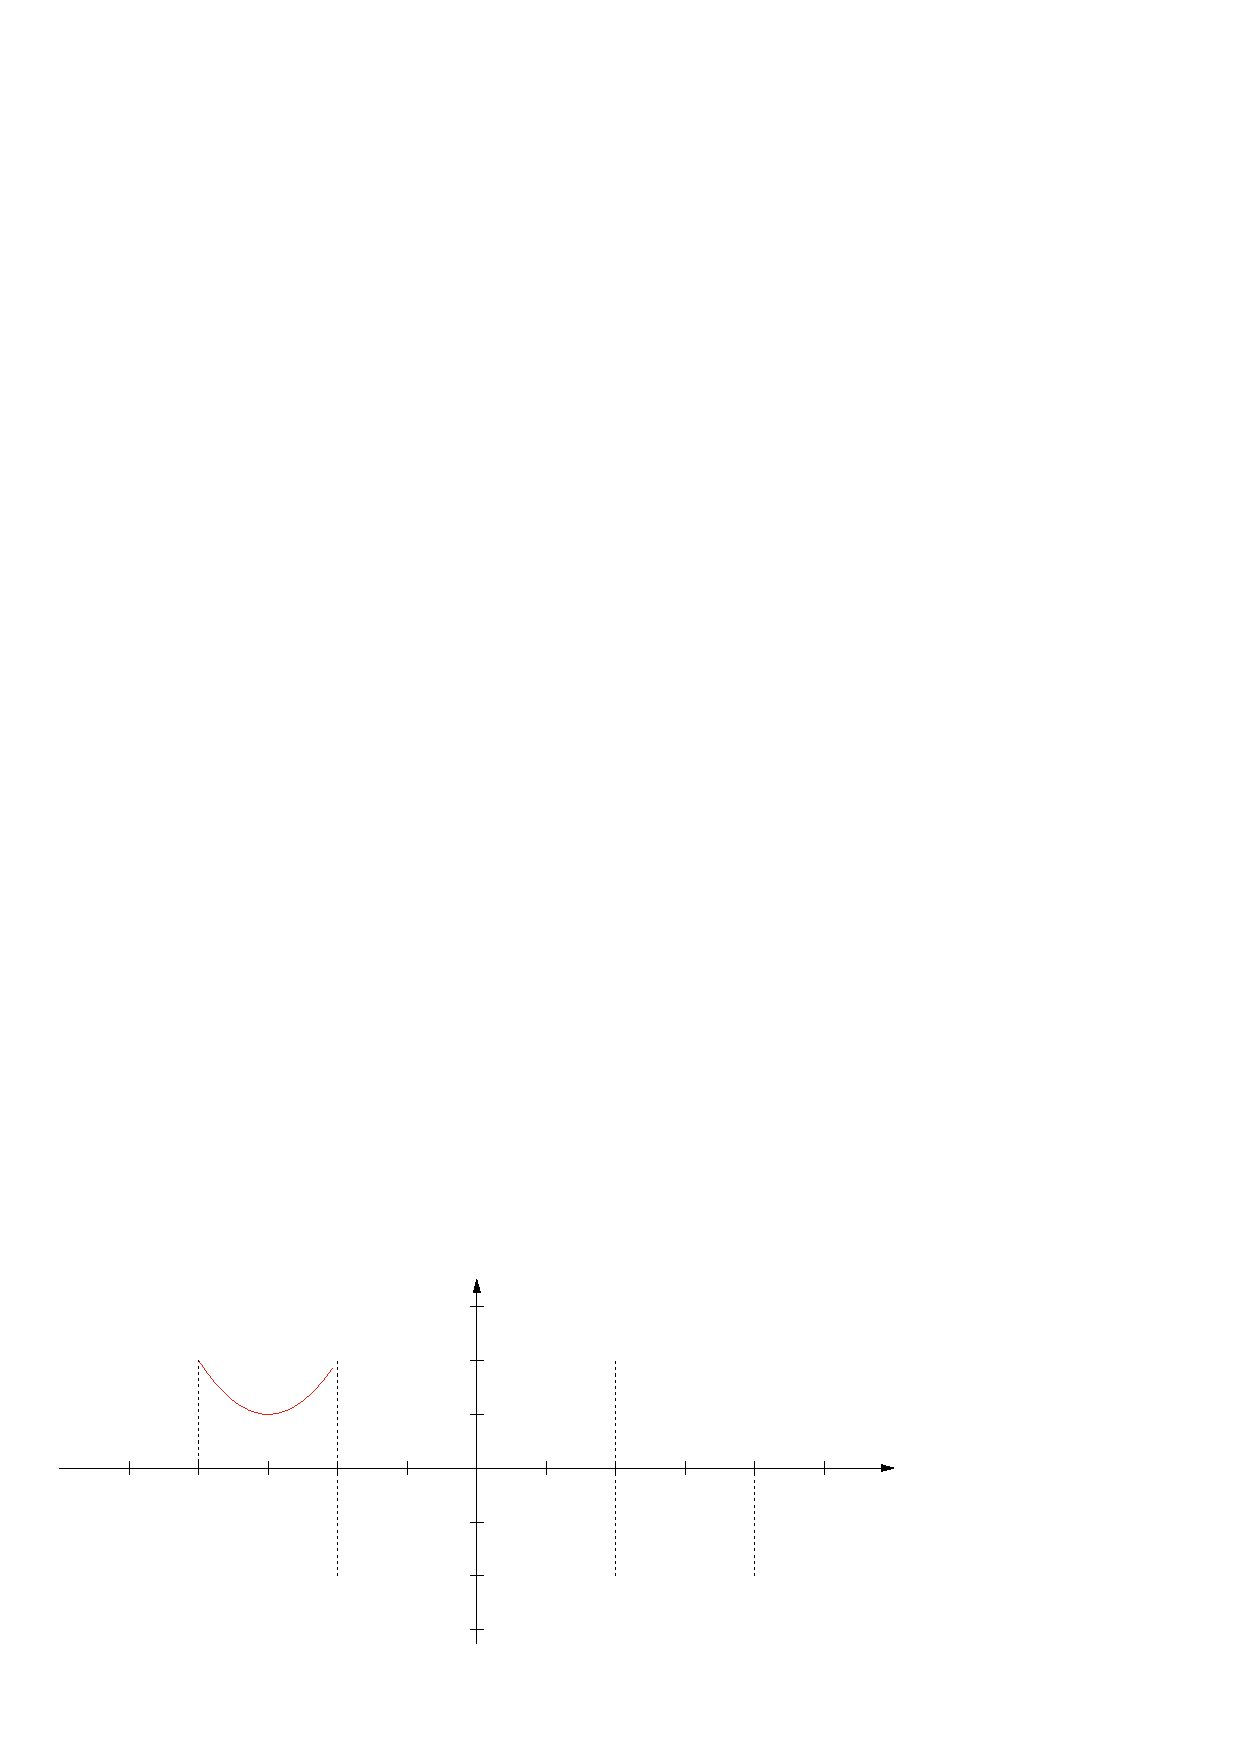
\includegraphics[width={360.00bp},height={172.80bp}]{figura_02_08}}%
    \gplfronttext
  \end{picture}%
\endgroup

\end{figure}

\subsection{Evaluación de coeficientes de \emph{Fourier}}
\subsubsection{Simetría de cuarto de onda par}
Como la función $f(t)$ tiene simetría de media onda:
\begin{equation}
    a_0=0
\end{equation}

Como la función $f(t)$ es una función par:
\begin{equation}
    b_n=0
\end{equation}

Como la función $f(t)$ tiene simetría de media onda: $a_n=0$ cuando $n$ es par.

Para $n$ impar:
\begin{equation*}
\begin{split}
    a_n
        &=\frac{4}{T}\int_0^{T/2} f(t)\cos(n\omega_0 t)\,dt\\
        &=\frac{4}{T}\left[
            \int_0^{T/4} f(t)\cos(n\omega_0 t)\,dt+
            \int_{T/4}^{T/2} f(t)\cos(n\omega_0 t)\,dt
        \right]\\
        &=\frac{4}{T}\left[
            \int_0^{T/4} f(t)\cos(n\omega_0 t)\,dt-
            \int_{T/4}^{T/2} f(t-\frac{T}{2})\cos(n\omega_0 t)\,dt
        \right]\\
\end{split}
\end{equation*}
\begin{equation*}
    \tau=t-\frac{T}{2}
\end{equation*}
\begin{equation*}
    d\tau=dt
\end{equation*}
\begin{equation*}
\begin{split}
    a_n
        &=\frac{4}{T}\left[
            \int_0^{T/4} f(t)\cos(n\omega_0 t)\,dt-
            \int_{\tau=T/4-T/2}^{\tau=T/2-T/2}
                f(\tau)\cos(n\omega_0(\tau+\frac{T}{2}))\,d\tau
        \right]\\
        &=\frac{4}{T}\left[
            \int_0^{T/4} f(t)\cos(n\omega_0 t)\,dt-
            \int_{-T/4}^{0} f(\tau)\cos(n\omega_0(\tau+\frac{T}{2}))\,d\tau
        \right]\\
\end{split}
\end{equation*}
\begin{equation*}
\begin{split}
    n\omega_0(\tau+T/2)
        &=n\omega_0\tau+n\omega_0\frac{T}{2}\\
        &=n\omega_0\tau+n\frac{2\pi}{T}\frac{T}{2}\\
        &=n\omega_0\tau+n\pi\\
\end{split}
\end{equation*}
\begin{equation*}
\begin{split}
    \cos(n\omega_0\tau+n\pi)
        &=\cos(n\omega_0\tau)\cos(n\pi)-\sen(n\pi)\sen(n\omega_0\tau)\\
        &=\cos(n\omega_0\tau)\cos(n\pi)\\
        &=-\cos(n\omega_0\tau)\\
\end{split}
\end{equation*}
\begin{equation*}
\begin{split}
    a_n
        &=\frac{4}{T}\left[
            \int_0^{T/4} f(t)\cos(n\omega_0 t)\,dt+
            \int_{-T/4}^0 f(\tau)\cos(n\omega_0\tau)\,d\tau
        \right]\\
        &=\frac{4}{T}\left[\int_{-T/4}^{T/4} f(t)\cos(n\omega_0 t)\,dt\right]\\
        &=\frac{4}{T}\left(2\int_0^{T/4} f(t)\cos(n\omega_0 t)\,dt\right)\\
        &=\frac{8}{T}\int_0^{T/4} f(t)\cos(n\omega_0 t)\,dt\\
\end{split}
\end{equation*}
\begin{equation}
\begin{cases}
    n: \text{par}   &a_n=0\\
    n: \text{impar} &a_n=\frac{8}{T}\int_0^{T/4}f(t)\cos(n\omega_0 t)\,dt\\
\end{cases}
\end{equation}

\subsubsection{Simetría de cuarto de onda impar}
Como la función $f(t)$ tiene simetría de media onda:
\begin{equation}
    a_0=0
\end{equation}

Como la función $f(t)$ es una función impar:
\begin{equation}
    a_n=0
\end{equation}

Como la función $f(t)$ tiene simetría de media onda: $b_n=0$ cuando $n$ es par.

Para $n$ impar:
\begin{equation*}
\begin{split}
    b_n
        &=\frac{4}{T}\int_0^{T/2} f(t)\sen(n\omega_0 t)\,dt\\
        &=\frac{4}{T}\left[
            \int_0^{T/4} f(t)\sen(n\omega_0 t)\,dt+
            \int_{T/4}^{T/2} f(t)\sen(n\omega_0 t)\,dt
        \right]\\
        &=\frac{4}{T}\left[
            \int_0^{T/4} f(t)\sen(n\omega_0 t)\,dt-
            \int_{T/4}^{T/2} f(t-\frac{T}{2})\sen(n\omega_0 t)\,dt
        \right]\\
\end{split}
\end{equation*}
\begin{equation*}
    \tau=t-\frac{T}{2}
\end{equation*}
\begin{equation*}
    d\tau=dt
\end{equation*}
\begin{equation*}
\begin{split}
    b_n
        &=\frac{4}{T}\left[
            \int_0^{T/4} f(t)\sen(n\omega_0 t)\,dt-
            \int_{\tau=T/4-T/2}^{\tau=T/2-T/2}
                f(\tau)\sen(n\omega_0(\tau+\frac{T}{2}))\,d\tau
        \right]\\
        &=\frac{4}{T}\left[
            \int_0^{T/4} f(t)\sen(n\omega_0 t)\,dt-
            \int_{-T/4}^{0}
                f(\tau)\sen(n\omega_0(\tau+\frac{T}{2}))\,d\tau
        \right]\\
\end{split}
\end{equation*}
\begin{equation*}
\begin{split}
    n\omega_0(\tau+T/2)
        &=n\omega_0\tau+n\omega_0\frac{T}{2}\\
        &=n\omega_0\tau+n\frac{2\pi}{T}\frac{T}{2}\\
        &=n\omega_0\tau+n\pi\\
\end{split}
\end{equation*}
\begin{equation*}
\begin{split}
    \sen(n\omega_0\tau+n\pi)
        &=\sen(n\omega_0\tau)\cos(n\pi)+\sen(n\pi)\cos(n\omega_0\tau)\\
        &=\sen(n\omega_0\tau)\cos(n\pi)\\
        &=-\sen(n\omega_0\tau)\\
\end{split}
\end{equation*}
\begin{equation*}
\begin{split}
    b_n
        &=\frac{4}{T}\left[
            \int_0^{T/4} f(t)\sen(n\omega_0 t)\,dt+
            \int_{-T/4}^0 f(\tau)\sen(n\omega_0\tau)\,d\tau
        \right]\\
        &=\frac{4}{T}\left[\int_{-T/4}^{T/4} f(t)\sen(n\omega_0 t)\,dt\right]\\
        &=\frac{4}{T}\left(2\int_0^{T/4} f(t)\sen(n\omega_0 t)\,dt\right)\\
        &=\frac{8}{T}\int_0^{T/4} f(t)\sen(n\omega_0 t)\,dt\\
\end{split}
\end{equation*}
\begin{equation}
\begin{cases}
    n: \text{par}   &b_n=0\\
    n: \text{impar} &b_n=\frac{8}{T}\int_0^{T/4}f(t)\sen(n\omega_0 t)\,dt\\
\end{cases}
\end{equation}

\section{Expansión periódica de funciones definidas en intervalos finitos}
Sea $f(t)$ una función no periódica:
\begin{figure}[H]
    \centering
    % GNUPLOT: LaTeX picture with Postscript
\begingroup
  \makeatletter
  \providecommand\color[2][]{%
    \GenericError{(gnuplot) \space\space\space\@spaces}{%
      Package color not loaded in conjunction with
      terminal option `colourtext'%
    }{See the gnuplot documentation for explanation.%
    }{Either use 'blacktext' in gnuplot or load the package
      color.sty in LaTeX.}%
    \renewcommand\color[2][]{}%
  }%
  \providecommand\includegraphics[2][]{%
    \GenericError{(gnuplot) \space\space\space\@spaces}{%
      Package graphicx or graphics not loaded%
    }{See the gnuplot documentation for explanation.%
    }{The gnuplot epslatex terminal needs graphicx.sty or graphics.sty.}%
    \renewcommand\includegraphics[2][]{}%
  }%
  \providecommand\rotatebox[2]{#2}%
  \@ifundefined{ifGPcolor}{%
    \newif\ifGPcolor
    \GPcolorfalse
  }{}%
  \@ifundefined{ifGPblacktext}{%
    \newif\ifGPblacktext
    \GPblacktexttrue
  }{}%
  % define a \g@addto@macro without @ in the name:
  \let\gplgaddtomacro\g@addto@macro
  % define empty templates for all commands taking text:
  \gdef\gplbacktext{}%
  \gdef\gplfronttext{}%
  \makeatother
  \ifGPblacktext
    % no textcolor at all
    \def\colorrgb#1{}%
    \def\colorgray#1{}%
  \else
    % gray or color?
    \ifGPcolor
      \def\colorrgb#1{\color[rgb]{#1}}%
      \def\colorgray#1{\color[gray]{#1}}%
      \expandafter\def\csname LTw\endcsname{\color{white}}%
      \expandafter\def\csname LTb\endcsname{\color{black}}%
      \expandafter\def\csname LTa\endcsname{\color{black}}%
      \expandafter\def\csname LT0\endcsname{\color[rgb]{1,0,0}}%
      \expandafter\def\csname LT1\endcsname{\color[rgb]{0,1,0}}%
      \expandafter\def\csname LT2\endcsname{\color[rgb]{0,0,1}}%
      \expandafter\def\csname LT3\endcsname{\color[rgb]{1,0,1}}%
      \expandafter\def\csname LT4\endcsname{\color[rgb]{0,1,1}}%
      \expandafter\def\csname LT5\endcsname{\color[rgb]{1,1,0}}%
      \expandafter\def\csname LT6\endcsname{\color[rgb]{0,0,0}}%
      \expandafter\def\csname LT7\endcsname{\color[rgb]{1,0.3,0}}%
      \expandafter\def\csname LT8\endcsname{\color[rgb]{0.5,0.5,0.5}}%
    \else
      % gray
      \def\colorrgb#1{\color{black}}%
      \def\colorgray#1{\color[gray]{#1}}%
      \expandafter\def\csname LTw\endcsname{\color{white}}%
      \expandafter\def\csname LTb\endcsname{\color{black}}%
      \expandafter\def\csname LTa\endcsname{\color{black}}%
      \expandafter\def\csname LT0\endcsname{\color{black}}%
      \expandafter\def\csname LT1\endcsname{\color{black}}%
      \expandafter\def\csname LT2\endcsname{\color{black}}%
      \expandafter\def\csname LT3\endcsname{\color{black}}%
      \expandafter\def\csname LT4\endcsname{\color{black}}%
      \expandafter\def\csname LT5\endcsname{\color{black}}%
      \expandafter\def\csname LT6\endcsname{\color{black}}%
      \expandafter\def\csname LT7\endcsname{\color{black}}%
      \expandafter\def\csname LT8\endcsname{\color{black}}%
    \fi
  \fi
    \setlength{\unitlength}{0.0500bp}%
    \ifx\gptboxheight\undefined%
      \newlength{\gptboxheight}%
      \newlength{\gptboxwidth}%
      \newsavebox{\gptboxtext}%
    \fi%
    \setlength{\fboxrule}{0.5pt}%
    \setlength{\fboxsep}{1pt}%
    \definecolor{tbcol}{rgb}{1,1,1}%
\begin{picture}(6336.00,2590.00)%
    \gplgaddtomacro\gplbacktext{%
      \csname LTb\endcsname%%
      \put(1233,416){\makebox(0,0)[r]{\strut{}}}%
      \put(1233,863){\makebox(0,0)[r]{\strut{}}}%
      \put(1233,1311){\makebox(0,0)[r]{\strut{}}}%
      \put(1233,1758){\makebox(0,0)[r]{\strut{}}}%
      \put(1233,2205){\makebox(0,0)[r]{\strut{}}}%
      \put(603,640){\makebox(0,0){\strut{}}}%
      \put(1329,640){\makebox(0,0){\strut{}}}%
      \put(2055,640){\makebox(0,0){\strut{}}}%
      \put(2781,640){\makebox(0,0){\strut{}}}%
      \put(3506,640){\makebox(0,0){\strut{}}}%
      \put(4232,640){\makebox(0,0){\strut{}}}%
      \put(4958,640){\makebox(0,0){\strut{}}}%
      \put(5684,640){\makebox(0,0){\strut{}}}%
      \csname LTb\endcsname%%
      \put(6228,863){\makebox(0,0)[l]{\strut{}$t$}}%
      \put(1502,2429){\makebox(0,0)[l]{\strut{}$f(t)$}}%
      \put(2681,662){\makebox(0,0)[l]{\strut{}$M$}}%
    }%
    \gplgaddtomacro\gplfronttext{%
    }%
    \gplbacktext
    \put(0,0){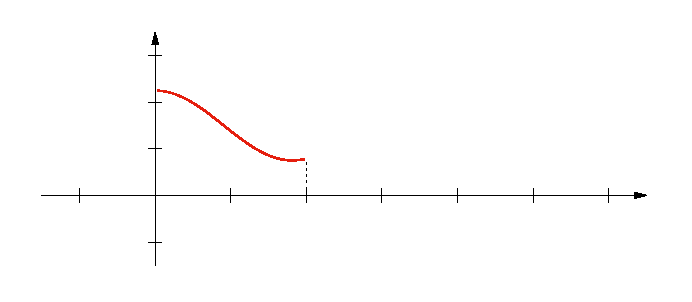
\includegraphics[width={316.80bp},height={129.50bp}]{figura_02_09}}%
    \gplfronttext
  \end{picture}%
\endgroup

\end{figure}

$f(t)$ se convierte en periódica al repetirla un intervalo $T\geq M$.
\begin{figure}[H]
    \centering
    % GNUPLOT: LaTeX picture with Postscript
\begingroup
  \makeatletter
  \providecommand\color[2][]{%
    \GenericError{(gnuplot) \space\space\space\@spaces}{%
      Package color not loaded in conjunction with
      terminal option `colourtext'%
    }{See the gnuplot documentation for explanation.%
    }{Either use 'blacktext' in gnuplot or load the package
      color.sty in LaTeX.}%
    \renewcommand\color[2][]{}%
  }%
  \providecommand\includegraphics[2][]{%
    \GenericError{(gnuplot) \space\space\space\@spaces}{%
      Package graphicx or graphics not loaded%
    }{See the gnuplot documentation for explanation.%
    }{The gnuplot epslatex terminal needs graphicx.sty or graphics.sty.}%
    \renewcommand\includegraphics[2][]{}%
  }%
  \providecommand\rotatebox[2]{#2}%
  \@ifundefined{ifGPcolor}{%
    \newif\ifGPcolor
    \GPcolorfalse
  }{}%
  \@ifundefined{ifGPblacktext}{%
    \newif\ifGPblacktext
    \GPblacktexttrue
  }{}%
  % define a \g@addto@macro without @ in the name:
  \let\gplgaddtomacro\g@addto@macro
  % define empty templates for all commands taking text:
  \gdef\gplbacktext{}%
  \gdef\gplfronttext{}%
  \makeatother
  \ifGPblacktext
    % no textcolor at all
    \def\colorrgb#1{}%
    \def\colorgray#1{}%
  \else
    % gray or color?
    \ifGPcolor
      \def\colorrgb#1{\color[rgb]{#1}}%
      \def\colorgray#1{\color[gray]{#1}}%
      \expandafter\def\csname LTw\endcsname{\color{white}}%
      \expandafter\def\csname LTb\endcsname{\color{black}}%
      \expandafter\def\csname LTa\endcsname{\color{black}}%
      \expandafter\def\csname LT0\endcsname{\color[rgb]{1,0,0}}%
      \expandafter\def\csname LT1\endcsname{\color[rgb]{0,1,0}}%
      \expandafter\def\csname LT2\endcsname{\color[rgb]{0,0,1}}%
      \expandafter\def\csname LT3\endcsname{\color[rgb]{1,0,1}}%
      \expandafter\def\csname LT4\endcsname{\color[rgb]{0,1,1}}%
      \expandafter\def\csname LT5\endcsname{\color[rgb]{1,1,0}}%
      \expandafter\def\csname LT6\endcsname{\color[rgb]{0,0,0}}%
      \expandafter\def\csname LT7\endcsname{\color[rgb]{1,0.3,0}}%
      \expandafter\def\csname LT8\endcsname{\color[rgb]{0.5,0.5,0.5}}%
    \else
      % gray
      \def\colorrgb#1{\color{black}}%
      \def\colorgray#1{\color[gray]{#1}}%
      \expandafter\def\csname LTw\endcsname{\color{white}}%
      \expandafter\def\csname LTb\endcsname{\color{black}}%
      \expandafter\def\csname LTa\endcsname{\color{black}}%
      \expandafter\def\csname LT0\endcsname{\color{black}}%
      \expandafter\def\csname LT1\endcsname{\color{black}}%
      \expandafter\def\csname LT2\endcsname{\color{black}}%
      \expandafter\def\csname LT3\endcsname{\color{black}}%
      \expandafter\def\csname LT4\endcsname{\color{black}}%
      \expandafter\def\csname LT5\endcsname{\color{black}}%
      \expandafter\def\csname LT6\endcsname{\color{black}}%
      \expandafter\def\csname LT7\endcsname{\color{black}}%
      \expandafter\def\csname LT8\endcsname{\color{black}}%
    \fi
  \fi
    \setlength{\unitlength}{0.0500bp}%
    \ifx\gptboxheight\undefined%
      \newlength{\gptboxheight}%
      \newlength{\gptboxwidth}%
      \newsavebox{\gptboxtext}%
    \fi%
    \setlength{\fboxrule}{0.5pt}%
    \setlength{\fboxsep}{1pt}%
    \definecolor{tbcol}{rgb}{1,1,1}%
\begin{picture}(6336.00,2590.00)%
    \gplgaddtomacro\gplbacktext{%
      \csname LTb\endcsname%%
      \put(1233,416){\makebox(0,0)[r]{\strut{}}}%
      \put(1233,863){\makebox(0,0)[r]{\strut{}}}%
      \put(1233,1311){\makebox(0,0)[r]{\strut{}}}%
      \put(1233,1758){\makebox(0,0)[r]{\strut{}}}%
      \put(1233,2205){\makebox(0,0)[r]{\strut{}}}%
      \put(603,640){\makebox(0,0){\strut{}}}%
      \put(1329,640){\makebox(0,0){\strut{}}}%
      \put(2055,640){\makebox(0,0){\strut{}}}%
      \put(2781,640){\makebox(0,0){\strut{}}}%
      \put(3506,640){\makebox(0,0){\strut{}}}%
      \put(4232,640){\makebox(0,0){\strut{}}}%
      \put(4958,640){\makebox(0,0){\strut{}}}%
      \put(5684,640){\makebox(0,0){\strut{}}}%
      \csname LTb\endcsname%%
      \put(6228,863){\makebox(0,0)[l]{\strut{}$t$}}%
      \put(1502,2429){\makebox(0,0)[l]{\strut{}$f(t)$}}%
      \put(2681,662){\makebox(0,0)[l]{\strut{}$M$}}%
      \put(2360,192){\makebox(0,0)[l]{\strut{}$T$}}%
    }%
    \gplgaddtomacro\gplfronttext{%
    }%
    \gplgaddtomacro\gplbacktext{%
      \csname LTb\endcsname%%
      \put(1233,416){\makebox(0,0)[r]{\strut{}}}%
      \put(1233,863){\makebox(0,0)[r]{\strut{}}}%
      \put(1233,1311){\makebox(0,0)[r]{\strut{}}}%
      \put(1233,1758){\makebox(0,0)[r]{\strut{}}}%
      \put(1233,2205){\makebox(0,0)[r]{\strut{}}}%
      \put(603,640){\makebox(0,0){\strut{}}}%
      \put(1329,640){\makebox(0,0){\strut{}}}%
      \put(2055,640){\makebox(0,0){\strut{}}}%
      \put(2781,640){\makebox(0,0){\strut{}}}%
      \put(3506,640){\makebox(0,0){\strut{}}}%
      \put(4232,640){\makebox(0,0){\strut{}}}%
      \put(4958,640){\makebox(0,0){\strut{}}}%
      \put(5684,640){\makebox(0,0){\strut{}}}%
      \csname LTb\endcsname%%
      \put(6228,863){\makebox(0,0)[l]{\strut{}$t$}}%
      \put(1502,2429){\makebox(0,0)[l]{\strut{}$f(t)$}}%
      \put(2681,662){\makebox(0,0)[l]{\strut{}$M$}}%
      \put(2360,192){\makebox(0,0)[l]{\strut{}$T$}}%
    }%
    \gplgaddtomacro\gplfronttext{%
    }%
    \gplgaddtomacro\gplbacktext{%
      \csname LTb\endcsname%%
      \put(1233,416){\makebox(0,0)[r]{\strut{}}}%
      \put(1233,863){\makebox(0,0)[r]{\strut{}}}%
      \put(1233,1311){\makebox(0,0)[r]{\strut{}}}%
      \put(1233,1758){\makebox(0,0)[r]{\strut{}}}%
      \put(1233,2205){\makebox(0,0)[r]{\strut{}}}%
      \put(603,640){\makebox(0,0){\strut{}}}%
      \put(1329,640){\makebox(0,0){\strut{}}}%
      \put(2055,640){\makebox(0,0){\strut{}}}%
      \put(2781,640){\makebox(0,0){\strut{}}}%
      \put(3506,640){\makebox(0,0){\strut{}}}%
      \put(4232,640){\makebox(0,0){\strut{}}}%
      \put(4958,640){\makebox(0,0){\strut{}}}%
      \put(5684,640){\makebox(0,0){\strut{}}}%
      \csname LTb\endcsname%%
      \put(6228,863){\makebox(0,0)[l]{\strut{}$t$}}%
      \put(1502,2429){\makebox(0,0)[l]{\strut{}$f(t)$}}%
      \put(2681,662){\makebox(0,0)[l]{\strut{}$M$}}%
      \put(2360,192){\makebox(0,0)[l]{\strut{}$T$}}%
    }%
    \gplgaddtomacro\gplfronttext{%
    }%
    \gplgaddtomacro\gplbacktext{%
      \csname LTb\endcsname%%
      \put(1233,416){\makebox(0,0)[r]{\strut{}}}%
      \put(1233,863){\makebox(0,0)[r]{\strut{}}}%
      \put(1233,1311){\makebox(0,0)[r]{\strut{}}}%
      \put(1233,1758){\makebox(0,0)[r]{\strut{}}}%
      \put(1233,2205){\makebox(0,0)[r]{\strut{}}}%
      \put(603,640){\makebox(0,0){\strut{}}}%
      \put(1329,640){\makebox(0,0){\strut{}}}%
      \put(2055,640){\makebox(0,0){\strut{}}}%
      \put(2781,640){\makebox(0,0){\strut{}}}%
      \put(3506,640){\makebox(0,0){\strut{}}}%
      \put(4232,640){\makebox(0,0){\strut{}}}%
      \put(4958,640){\makebox(0,0){\strut{}}}%
      \put(5684,640){\makebox(0,0){\strut{}}}%
      \csname LTb\endcsname%%
      \put(6228,863){\makebox(0,0)[l]{\strut{}$t$}}%
      \put(1502,2429){\makebox(0,0)[l]{\strut{}$f(t)$}}%
      \put(2681,662){\makebox(0,0)[l]{\strut{}$M$}}%
      \put(2360,192){\makebox(0,0)[l]{\strut{}$T$}}%
    }%
    \gplgaddtomacro\gplfronttext{%
    }%
    \gplbacktext
    \put(0,0){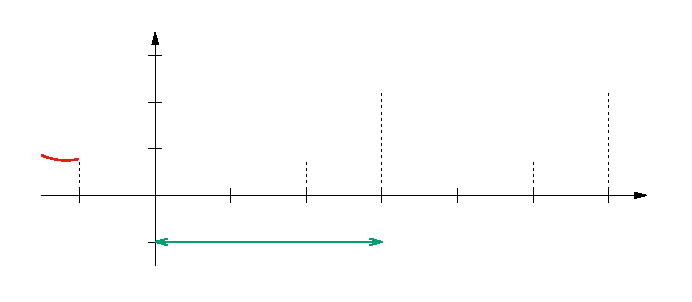
\includegraphics[width={316.80bp},height={129.50bp}]{figura_02_10}}%
    \gplfronttext
  \end{picture}%
\endgroup

\end{figure}

$f(t)$ puede expandirse periódicamente asignando alguna simetría conocida.

